\documentclass[conference,compsoc]{IEEEtran}

\IEEEoverridecommandlockouts

\usepackage[backend=bibtex]{biblatex}
\usepackage{unicode-math}
\usepackage{graphicx}
\usepackage{float}
\usepackage{url}

\addbibresource{references/references.bib}
\graphicspath{{./images/}}
\nocite{*}
\sloppy

\begin{document}

\title{Therabot - Your Pocket Therapist}

\author{\IEEEauthorblockN{Raja Rajan A}
\IEEEauthorblockA{Dayananda Sagar College of Engg.\\
Bengaluru, Karnataka, India\\
Email: im.amruth@gmail.com}
\and
\IEEEauthorblockN{Varsha Jambunathan}
\IEEEauthorblockA{Dayananda Sagar College of Engg.\\
Bengaluru, Karnataka, India\\
Email: jvarsha621@gmail.com}
\and
\IEEEauthorblockN{Laasya R.}
\IEEEauthorblockA{Dayananda Sagar College of Engg.\\
Bengaluru, Karnataka, India\\
Email: laasyadolly@gmail.com}}

\maketitle

\begin{abstract}
This study aims to highlight the use cases of a variety of technologies in the field of Artificial Intelligence, Speech Synthesis, Personalization, User Character Segmentation and Automated Text/Speech-based Chatbots. To illustrate the uses, we have chosen a specific field of expertise, mental wellness. We have built an artificially chatbot that is designed to understand the complexities of it’s user, help the user feel more self-aware and spontaneously check back on the user from time to time.
\end{abstract}

%% Introduction

\section{Introduction}

\subsection{The State of Mental Health}

Burden of mental disorders had risen over last few decades. Mental health is a state of well-being in which the individual realizes his or her own abilities, can cope with the normal stresses of life, can work productively and is able to make a contribution to his or her community. WHO estimated that globally over 450 million people suffer from mental disorders. Currently mental and behavioural disorders account for about 12 percent of the global burden of diseases. Major proportions of mental disorders come from low and middle income countries.

\begin{figure}[H]
    \centering
    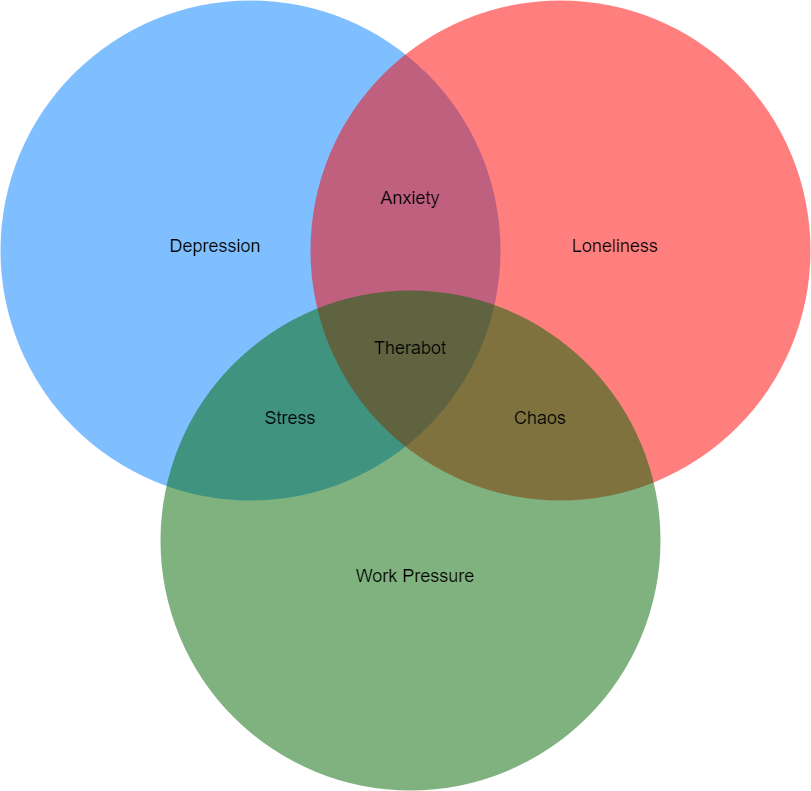
\includegraphics[width=6cm]{images/roots-mental-health-issues.png}
    \caption{Roots of Mental Health Issues}
    \label{fig:roots-mental-health-issues}
\end{figure}

Progress in mental health service delivery has been slow in most low- and middle-income countries. Barriers include the existing public-health priorities and its influence on funding; challenges to delivery of mental health care in primary-care settings; the low numbers of those trained in mental health care; and the lack of mental health perspective in public-health leadership.

Thus, it becomes now opportune to explore the paradigm of mental health awareness as a means of combating stigma, enhancing prevention, ensuring early recognition, and also stimulating simple and practical interventions within the community. Today there are opportunities in terms of growing acknowledgement of mental disorders as key targets of global health action, as well as of leveraging new technologies particularly internet, big data and cell phones in amplifying simple field interventions found successful in primary care and other echelons.

\subsection{The Cognitive Behavioural Therapy}

Cognitive behavioral therapy (CBT) is a short-term therapy technique used by counselors and therapists to teach individuals to change their unwanted behaviors by changing their thought patterns. The premise of cognitive behavioral therapy is that our thought patterns (cognition) and interpretations of life events greatly influence how we behave and, ultimately, how we feel.

\begin{figure}[H]
    \centering
    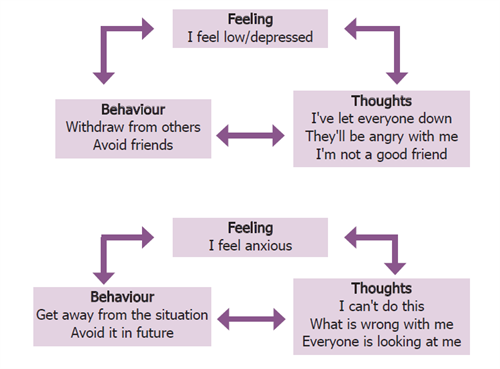
\includegraphics[width=6cm]{images/cbt-diagram.jpg}
    \caption{Sequence of Cognitive Behavioural Therapy}
    \label{fig:cbt-diagram}
\end{figure}

CBT is a form of psychotherapy that focuses on how your thoughts, beliefs and attitudes affect your feelings and behavior. It aims to teach you effective coping strategies for dealing with different problems throughout life. CBT can help you make sense of overwhelming problems by breaking them down into smaller parts.

One of the key tenets of CBT is that distorted thinking leads to distress and problematic behaviors, whereas thinking realistically with less negativity allows individuals to respond to challenging life circumstances in an effective way. Research shows this technique is an effective therapy for not only depression and panic disorder, but many illnesses and dysfunctional behaviors.

\subsection{The Rise of Chatbots}

A chatbot is one of the simple ways to transport data from a computer without having to think for proper keywords to look up in a search or browse several web pages to collect information; users can easily type their query in natural language and retrieve information. In this paper, information about the design, implementation of the chatbot has been presented.

From the survey above, it can be said that the development and improvement of chatbot design grow at an unpredictable rate due to variety of methods and approaches used to design a chatbot. Chatbot is a great tool for quick interaction with the user. They help us by providing entertainment, saving time and answering the questions that are hard to find. The Chatbot must be simple and conversational. Since there are many designs and approaches for creating a chatbot, it can be at odds with commercial considerations. Researchers need to interact and must agree on a common approach for designing a Chatbot.

In this project, we looked into how chatbots are developed and the applications of chatbots in various fields. In addition, comparison has been made with other chatbots in the same field of interest. A general purpose chatbot must be simple, user friendly, must be easily understood and the knowledge base must be compact. Although some of the commercial products have recently emerged, improvements must be made to find a common approach for designing a chatbot.

Chatbots have seen a huge rise in the recent markets and have primarily been used in the fields of service, question and answering and quite recently, home automation. They have proven to be very useful in the field of automation and have successfully replaced menial jobs that could’ve cost a lot of money for major corporations. Current commercial chatbots are capable of understanding simple sentences through pattern matching techniques, and search for questions asked in a repository of answers. This works out well in a closed scenario where the kind of questions the user may ask are limited, but not in a real life scenario.

\begin{figure}[H]
    \centering
    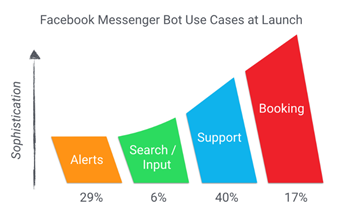
\includegraphics[width=6cm]{images/chatbot-usecases.png}
    \caption{Usecases of Chatbots}
    \label{fig:chatbot-usecases}
\end{figure}

Chatbots were later trained on neural networks to become much smarter, using a larger dataset. They were trained to learn on a wider spectrum and can understand sentences in a more humane form due to the advancements in NLP. But with all the new things that chatbots now have to learn, they’ve never really been personal to an individual.

\begin{figure}[H]
    \centering
    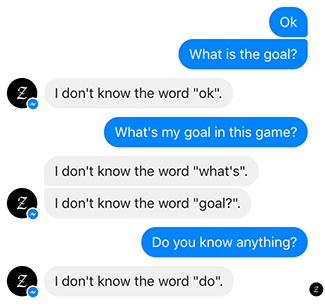
\includegraphics[width=6cm]{images/dumb-chatbot.png}
    \caption{Dumb Chatbots}
    \label{fig:dumb-chatbot}
\end{figure}

The objective of our method is to create a personalized user model that is unique to every user but keeps them anonymous at the same time. This helps the chatbot response generator understand who the user is and push relatable content and context when necessary.

\subsection{The Abstract of Artificial Intelligence}

Artificial Intelligence (AI) is defined as intelligence exhibited by an artificial entity to solve complex problems and such a system is generally assumed to be a computer or machine. Artificial Intelligence is an integration of computer science and physiology Intelligence in simple language is the computational part of the ability to achieve goals in the world. Intelligence is the ability to think to imagine creating memorizing and understanding, recognizing patterns, making choices adapting to change and learn from experience.

\begin{figure}[H]
    \centering
    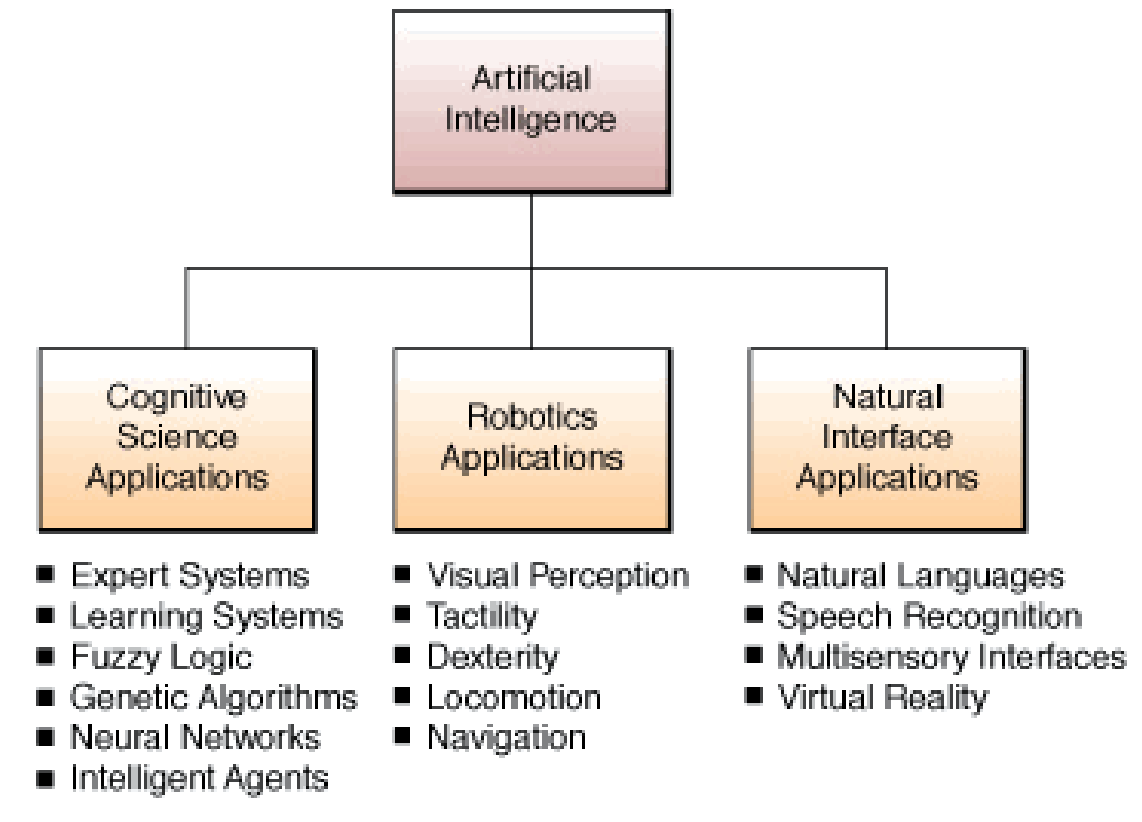
\includegraphics[width=6cm]{images/ai-overview.png}
    \caption{Overview of Artificial Intelligence}
    \label{fig:ai-overview}
\end{figure}

Artificial Intelligence was created with the sole aim of mimicking or even outperforming human minds. Thus it is very important we question the fact whether it has actually been able to do so.

It cannot be ignored that the fact of AI is being used all around us especially in the fields of medicine, robotics, law, stock trading etc. It is being used in homes and big establishments. such as military bases and the NASA space station. NASA has sent out artificially intelligent robots to planets so as to learn more about their habitat and atmosphere, with the intention of investigating if there is a possibility of humans living on these planets.

Expert systems have been used by Mercedes Benz and other auto manufacturers in the design of vehicle components, subway systems in Washington, D.C. use expert system software controllers to cause subway trains to stop within 3 inches of the right spot on the platform. These trains have motormen primarily to reassure passengers. AI has filtered into general applications in these fields and has become so common that it is not referred to as Artificial Intelligence anymore.

Blind supporters of AI would point to the time when AI Deep Blue II defeated chess master Garry Kasparov to prove that Artificial Intelligence can in fact be smarter than humans. Though there is no doubt that the AI Deep Blue II won that game, it is still probably one of the dumbest software alive. The operators were programming the AI in every round depending on the opposition’s last move. Also, the Deep Blue II had studied all of Kasparov’s previous games while the latter wasn’t given the same benefit. One can safely say that even though the Deep Blue II AI defeated Kasparov, it was never a fair fight to begin with. Latest technologies like Xbox 360’s Kinect and iPhone’s Siri use algorithms based on Artificial Intelligence, but it is a well-known fact that these technologies are a long way from being perfect.

Thus we can safely conclude that though Artificial Intelligence has made a lot of progress in the past few decades, it is not at a level where in one can confidently state that it is now ready to completely replace the human mind. That being said, large scale research is now being conducted into the field of proper simulation of the human brain.

%% Problem Statement

\section{Problem Statement and Proposed Solution}

\subsection{Problem Statement}

Narrative therapy is embracing into the second decade on the arena of psychotherapy. Yet, how can these therapeutic qualities best be inferred? How persuasive are the arguments relating to its effectiveness? What type of work is presides over with patients that portray that such practices are indeed beneficial to people? And lastly, how solid is the narrative-inspired research(often called co-research) that forge the use of externalizing practices? A distinctive quality of the therapeutic stance, if narrative therapy lies in the manner in which it pledges from the postmodern philosophical tradition. Similarly, narrative-based research pop up to be unique from other genre of research in mental health professions.

Conventional forms of research generally search for empirical conclusions (as with quantitative designs) and consistently rely on the researcher’s expert role to collect, codify, and interpret data (as is the case with many forms of qualitative methodology). Narrative-inspired research, conversely, limelight’s on the subjective nature of experience and inquire to de-emphasize the therapist’s role as an expert.

The relevant elements necessary for a basic psychotherapy reading, is:
\begin{itemize}
    \item What the main problem is (for example depression or anxiety).
    \item What triggers it (what makes the patient feel that way on a day to day basis).
    \item Examples of patient's symptoms, changes in patients behaviours and thinking.
    \item What consequence the problem has on patient's life.
\end{itemize}

An example with all the relevant elements needed, is:
``My main problem is feeling depressed most of the day every day. I feel tired, my Appetite is affected and I struggle to concentrate. I have stopped seeing friends, goingto work or doing things around the home and I am spending more time in bed. I have thoughts that I am letting my family down and that I can't be bothered. As a Consequence, I am isolated and being off sick means I have used up most of my savings and money is tight''.

\subsection{Existing State of the Art}

\begin{figure}[H]
    \centering
    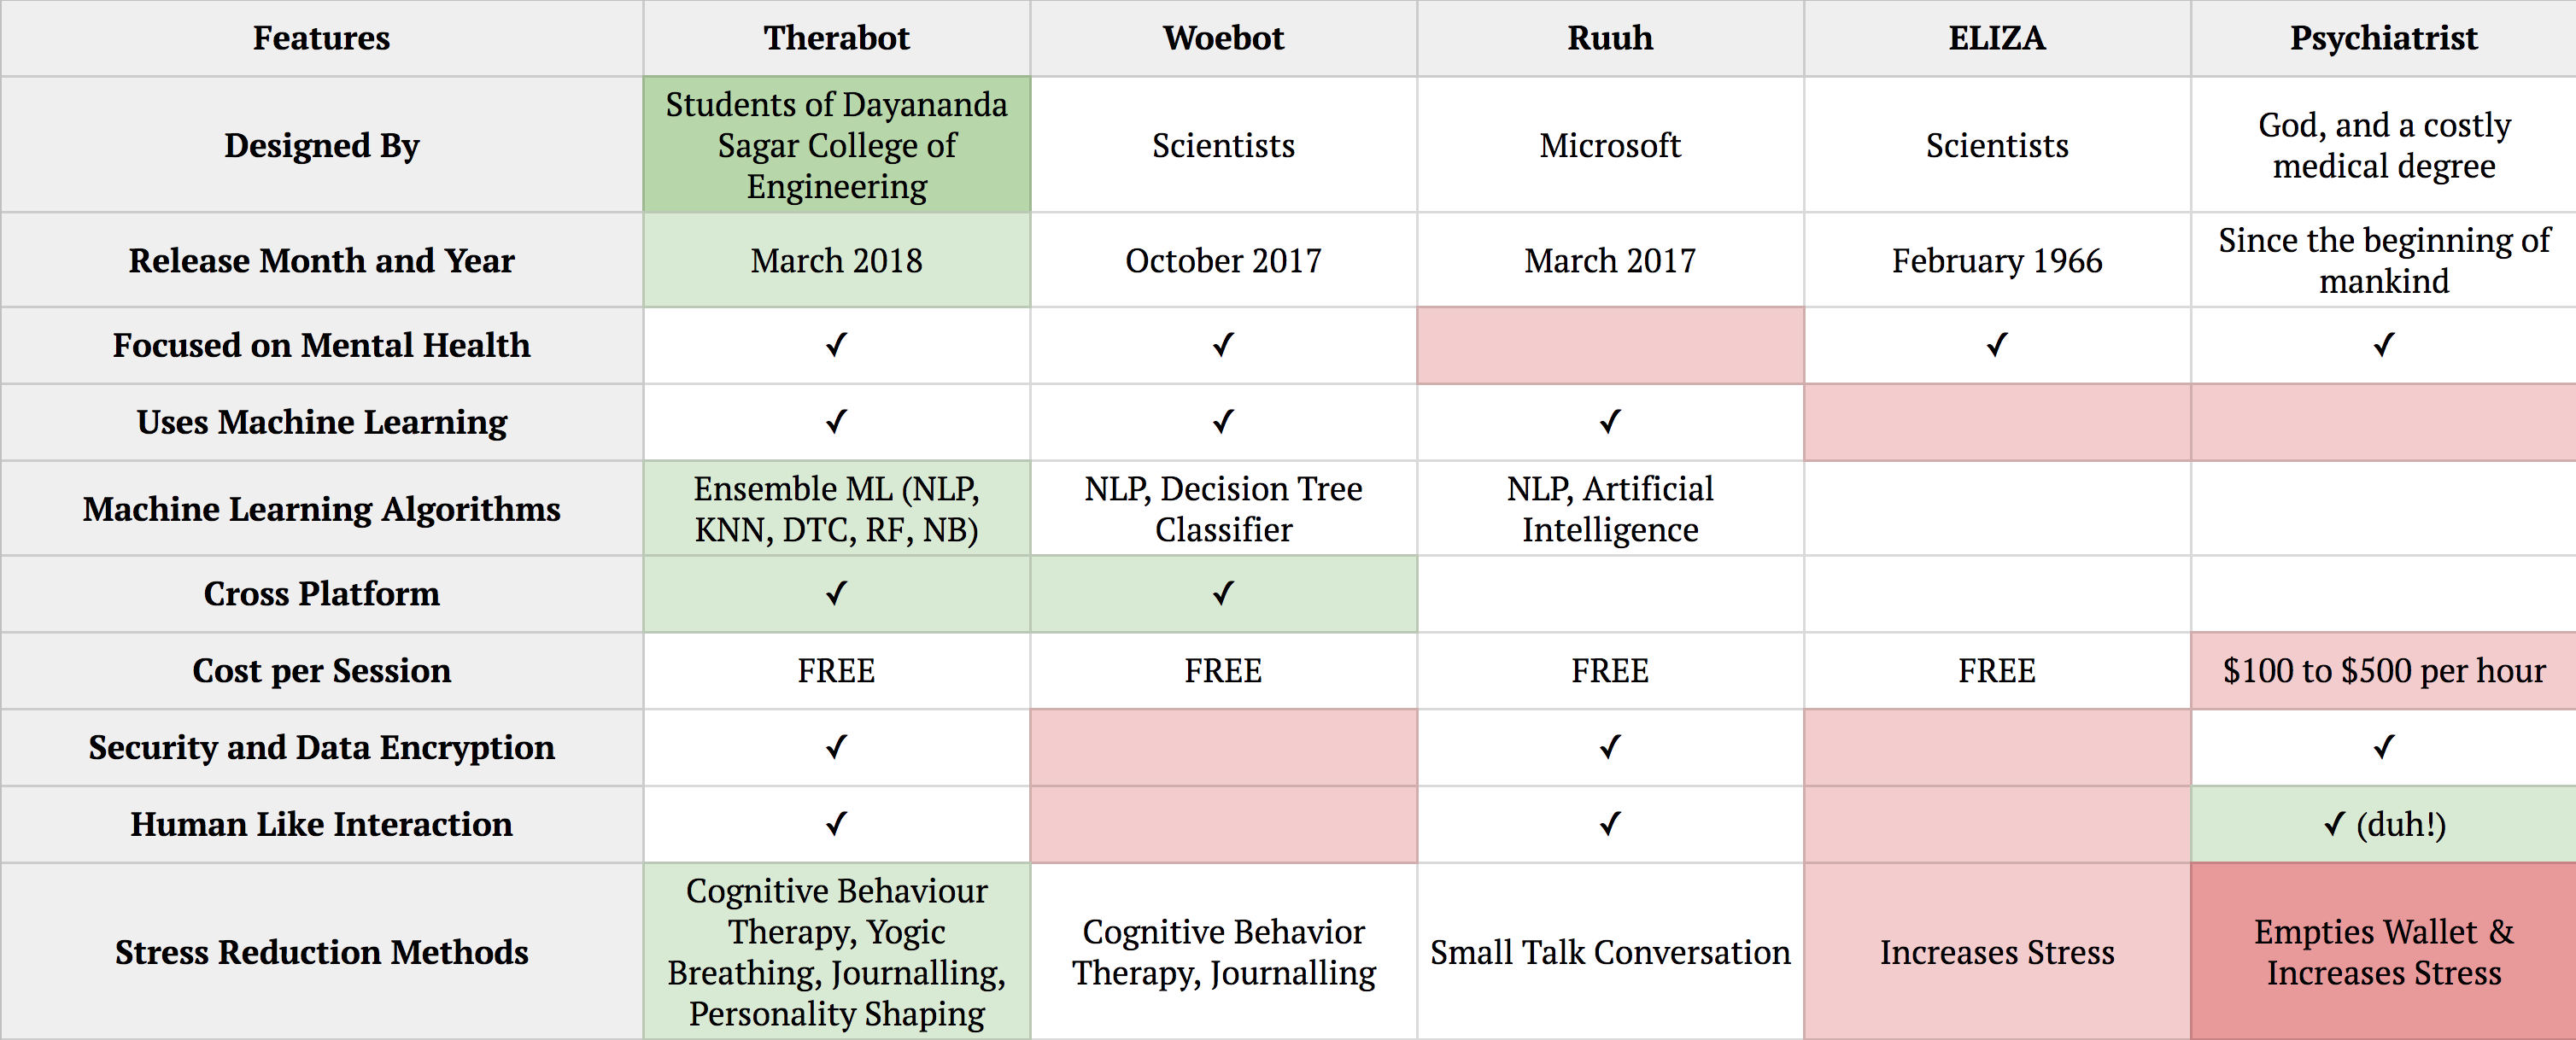
\includegraphics[width=6cm]{images/comparitive-study-of-competitors.png}
    \caption{Comparitive Study of Competitors}
    \label{fig:comparitive-study-of-competitors}
\end{figure}

Currently, people who do feel sad have only a handful of options available to them, including talking to friends, talking to family or seeing a therapist. The two are subjective, and doesn’t really apply when someone is clinically depressed and not willing to talk it out to his/her nearest and dearest.

Then, there are those who are hesitant to talk to strangers as well, considering they have the time and money to book an appointment with a therapist. Even if they do so, they have trouble opening up to someone who they have never met before.

When it comes to the existing Chatbot ecosystem, it has boomed in the market just a few days ago and has been dominant amongst companies to work as a front for their customer services portals, replacing everyday queries etc. We wanted to extend this functionality into something even more helpful and personal.

(why therapy, why chatbots) = (how good have they been : they trick the user into thinking that they are communicating with an actual person) chatbot which automatically gives immediate responses to the users based on the data set of Frequently Answered Questions (FAQs), using Artificial Intelligence Markup Language (AIML) and Latent Semantic Analysis (LSA). Template based questions like greetings and general questions will be answered using AIML and other service related questions use LSA to give responses.

\subsection{Proposed Solution}

The purpose of this study is to take an in-depth critical look into the narrative practice of externalizing; focusing intimately on its various uses and purported therapeutic qualities. The oneness of this deliberation is in the singular idiosyncrasy in which it locus on the various shot in which externalizing praxis are employed within narrative therapy and the leeway to which they are evaluated through research.

Narrative therapy proffer vast innovative essence and therapeutic practices. Key betwixt them is the praxis of engaging people in externalizing gab. Intermittently viewed as matter-of-factly a therapy technique, externalizing practices address wider inference about how clinicians view the world, understand clients quandary, and by association, how clients view their self and their potentiality to make turnover in their lives.

An evolving frame of narrative-inspired literature and research is being ordain that may assist in repose narrative therapy alongside other catalog and researched therapeutic entrance. An nonpartisan of this study is to further that literary process, concretely as it relates to the practice of externalizing. This study’s oneness lies in the comportment in which it targets solely on the issues and therapeutic entanglement surrounding externalizing practices. By doing this, it represents novel work in the field of narrative therapy literature, and will assist in explaining a pivotal narrative practice to the preponderant clinical psychology community.

The intent of this abstraction is to take an in-depth critical look into the narrative practice of externalizing; focusing intimately on its diversified uses and purported therapeutic qualities.

A considerable measure of literature abide on the multiple distinctive ways in which externalizing practices function. Much of the literature is sprinkled with various tantalizing therapeutic qualities ascribing to externalizing practices, often not beyond the context of how externalizing serves other narrative practices; such as deconstructive listening, reliant influence questions, discovering unique sequel, etc.

Accordingly, the oneness of this study is in the singular manner in which it locus on the numerous ways in which externalizing practices are employed within narrative therapy and the leeway to which they are evaluated through research.

Narrative therapy affirms many innovative ideas and therapeutic convenance. Key among them is the process of engaging people in externalizing interactions. consistently it is viewed as simply, a therapy technique, externalizing practices address wider implications about how clinicians picture the world, understand clients’ problems, and by association, how clients view themselves and their ability to make a new revision to their lives.

While narrative-inspired texts discept externalizing practices to varying degrees, this study is distinguished by the manner in which it locus singularly on the use of and therapeutic value concord with externalizing practices. By doing so, this study provides a richer forbearing of the theory and convention of externalizing approaches to clinicians versed in narrative work, as well as to those new to the narrative advent. It also intends an opportunity to explore in-depth the sequence of research behind narrative therapy and externalizing practices.

\subsection{Unique Features}
\begin{itemize}
    \item Build a simple and interactive real time chat system.
    \item Extraction of preferences and interests of the user.
    \item Dedicated system which is able be a bolster of support and understanding.
    \item Designed in such a way that it should work in cross platform devices.
    \item Effective hybrid models built on ensemble methods for reedy prediction.
    \item Can be easily integrated and upgradable.
\end{itemize}

\subsection{System Requirements}
\begin{itemize}
    \item Android/iOS Mobile Device to test/run the chatbot
    \item Facebook Messenger or Google Assistant
    \item Adequately fast Internet connection to access
    \begin{itemize}    
        \item Dialogflow
        \item Actions on Google Dashboard
        \item Firebase Firestore Database
        \item Google Cloud Platform Dashbaord
    \end{itemize}
    \item Node and NPM to run the webhook server
    \item Python 3.6+ to run the NLP and Analytics module
    \item iPython Notebook to test/run the scripts
    \item Flask to run the API server to access Python scripts
\end{itemize}

% Literature Survey

\section{Literature Survey}

\subsection{Base Papers}

\subsubsection{Engineering Base Paper}

\noindent
\textbf{Psychology Predictive Model Research based on Artificial Neural Network}

\noindent
\textit{\textbf{Author:} Cai Zhongxi}

Understanding the psychological state of mind in college students has become crucial due to the increasing mental health issues. The scenario is such that students succumb to emotional stress, learning pressure, relationship issues and inability to express thoughts, and are trapped in depression. This paper focuses on analyzing the incidents that affect the mental status of students by predicting the correlation between the implicating factors. The neural network is trained using a multilayer perceptron to obtain a back propagated output which needs optimization. The authors have proposed a mathematical model for the use of genetic algorithms to improve the mutation rate of the result, thereby, increasing the learning rate.

\subsubsection{Medical Base Paper}

\noindent
\textbf{Delivering Cognitive Behavior Therapy to Young Adults With Symptoms of Depression and Anxiety Using a Fully Automated Conversational Agent (Woebot):A Randomized Controlled Trial}

\noindent
\textit{\textbf{Authors:} Kathleen Kara Fitzpatrick, Alison Darcy and Molly Vierhile}

This paper outlines the role of Cognitive Behavior Therapy (CBT) in the treatment of individuals facing anxiety, depression, obsessive compulsive disorder (OCD), post-traumatic stress disorder (PTSD) and anger problems. The authors have created a chatterbot, Woebot, whose sole purpose is to talk to the user and get inputs about his mood. Patient Health Questionnaire-9 and Generalized Anxiety Disorder-7 are some of the standardized questionnaires that every therapist uses to determine the depression severity and frequency. Woebot uses these measures to better understand the individual.

\subsection{Additional Papers found through in-depth research}

\noindent
\textbf{Content-Oriented User Modeling for Personalized Response Ranking in Chatbots}

\noindent
\textit{\textbf{Authors:} Bingquan Liu , Zhen Xu , Chengjie Sun, Baoxun Wang , Xiaolong Wang, Derek F. Wong , Senior Member and Min Zhang}

Automatic chatbots (also known as chat-agents) have attracted much attention from both researching and industrial fields. Generally, the semantic relevance between users’ queries and the corresponding responses is considered as the essential element for conversation modeling in both generation and ranking based chat systems. This paper aims to address the personalized response ranking task by incorporating user profiles into the conversation model.\\

\noindent
\textbf{On the Construction of more Human-like Chatbots: Affect and Emotion Analysis of Movie Dialogue Data}

\noindent
\textit{\textbf{Author:} Rafael E. Banchs}

Affect and emotion are inherent properties of human-human communication and interaction. Recent research interest in chatbots and conversational agents aims at making human-machine interaction more human-like in both behavioral and attitudinal terms. This paper intends to present some baby steps in this direction by analyzing a large dialogue dataset in terms of tonal, affective and emotional bias, with the objective of providing a valuable resource for developing and training data-driven conversational agents with discriminative power across such dimensions.\\

\noindent
\textbf{NLAST: A natural language assistant for students}

\noindent
\textit{\textbf{Authors:} Fernando A. Mikic Fonte, Martín Llamas Nistal, Juan C. Burguillo Rial, and Manuel Caeiro Rodríguez}

This paper presents a system that works as an assistant for students in their learning process. The assistant system has two main parts: an Android application and a server platform. The Android application is a chatterbot (i.e., an agent intended to conduct a conversation in natural language with a human being) based on AIML, one of the more successful languages for developing conversational agents. The chatterbot acts as an intermediation agent between a student and the server platform.\\

\noindent
\textbf{Sentiment Analysis of Text using Deep Convolution Neural Networks}

\noindent
\textit{\textbf{Authors:} Anmol Chachra, Pulkit Mehndiratta and Mohit Gupta}

Sentiment analysis has been one of the most researched topics in Machine learning. The roots of sentiment analysis are in studies on public opinion analysis at the start of 20th century, but the outbreak of computer-based sentiment analysis only occurred with the availability of subjective text in Web. The task of generating effective sentence model that captures both syntactic and semantic relations has been the primary goal to make better sentiment analyzers. In this paper, we harness the power of deep convolutional neural networks (DCNN) to model sentences and perform sentiment analysis.\\

\noindent
\textbf{Big data in psychology: using word embeddings to study theory-of-mind}

\noindent
\textit{\textbf{Authors:} Michel Généreux, Bryor Snefjella and Marta Maslej}

This paper uses a computational approach to estimate the concreteness of words. After examining its reliability and validity, we apply this approach to study a claim within Psychology, namely, that reading a literary fiction story improves the ability to attribute mental states to others.\\

\noindent
\textbf{Automated Text Messaging as an Adjunct to Cognitive Behavioral Therapy for Depression:A Clinical Trial}

\noindent
\textit{\textbf{Authors:} Adrian Aguilera, Emma Bruehlman-Senecal, Orianna Demasi and Patricia Avila}

Cognitive Behavioral Therapy (CBT) for depression is efficacious, but effectiveness is limited when implemented in low-income settings due to engagement difficulties including nonadherence with skill-building homework and early discontinuation of treatment. Automated messaging can be used in clinical settings to increase dosage of depression treatment and encourage sustained engagement with psychotherapy.\\

\noindent
\textbf{Weighted Word2Vec Based on the Distance of Words}

\noindent
\textit{\textbf{Authors:} Chia-Yang Chang, Shie-Jue Lee and Chih-Chin Lai}

Word2vec is a novel technique for the study and application of natural language processing(NLP). It trains a word embedding neural network model with a large training corpus. After the model is trained, each word is represented by a vector in the specified vector space. The vectors obtained possess many interesting and useful characteristics that are implicitly embedded with the original words. The idea of word2vec is that there are relations between the words if they appear in the neighborhood.\\

% Architecture and Design

\section{Architecture and Design}

\subsection{System Overview}

The system is designed in such a way that it contains three main modules:
\begin{itemize}
    \item User Interface
    \item Natural Language Processing
    \item Sentiment \& Keyword Extraction
\end{itemize}

\subsubsection{User Interface}

We’ve integrated the Facebook Messenger and Google Assistant interface to be able to get into an array of devices right away instead of marketing to install a new application. The benefits to this is that, we would not take up any extra space on the user’s phone and also that there are zero to none chances of being hacked or reverse engineered since everything is on the server side and not on the client side which is under user control.

\subsubsection{Natural Language Processing}

This happens in realtime as we are conversing with the chatbot. The sentences being sent to the NLP module are broken down and tokenized into various parts of speech tags. These help the model understand what the significance of each word means. We will then attempt to match the key word to one of the intents in our database through means of similarity. If there exists no such match, we will simply call the Default Fallback Intent and display to the user that it doesn’t know what to do.

\subsubsection{Sentiment \& Keyword Extraction}

In this phase, we attempt to summarize the journals written by the user and extract the sentiment of the message. This will explain a lot about the user’s intent and interests, not to mention the dislikes. This information can be stored for each individual user and later used in casual conversations.

\subsection{Software Architecture}

First, architecture defines software elements. The architecture embodies information about how the elements relate to each other. This
means that it specifically omits certain information about elements that does not pertain to their interaction. Thus, an architecture is
foremost an abstraction of a system that suppresses details of elements that do not affect how they use, are used by, relate to, or interact
with other elements. In nearly all modern systems, elements interact with each other by means of interfaces that partition details about an
element into public and private parts. Architecture is concerned with the public side of this division; private details—those having to do
solely with internal implementation—are not architectural.

\subsubsection{System Block Diagram}

\begin{figure}[H]
    \centering
    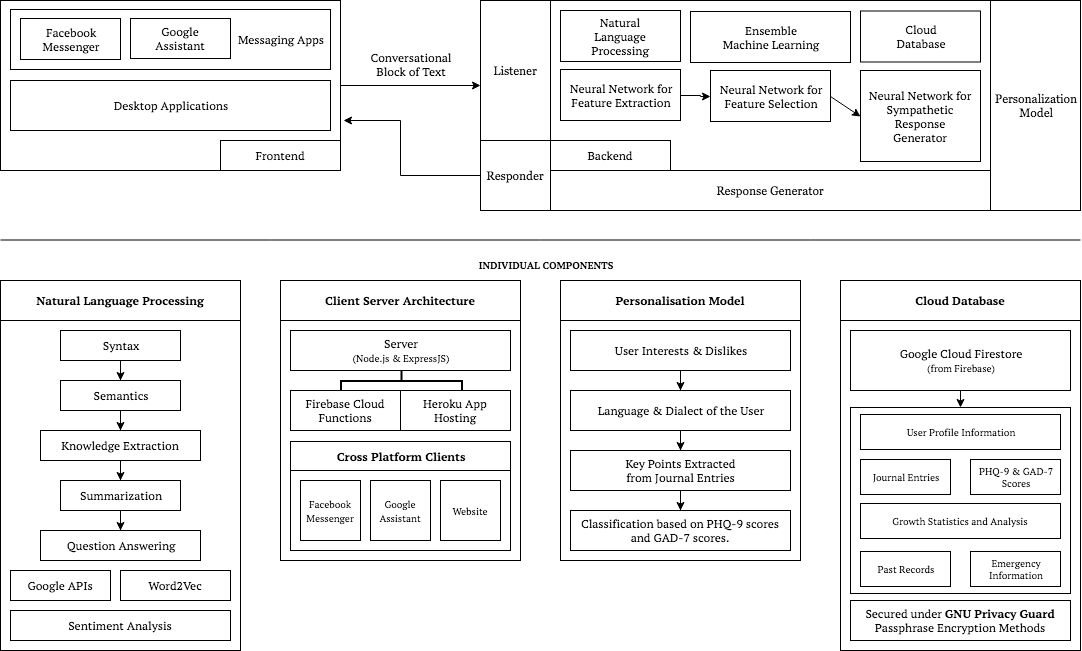
\includegraphics[width=6cm]{images/system-block-diagram.png}
    \caption{End-to-End System Block Diagram}
    \label{fig:system-block-diagram}
\end{figure}

Second, the definition makes clear that systems can and do comprise more than one structure and that no one structure can irrefutably
claim to be the architecture. For example, all nontrivial projects are partitioned into implementation units; these units are given specific
responsibilities and are frequently the basis of work assignments for programming teams. This type of element comprises programs and
data that software in other implementation units can call or access, and programs and data that are private. In large projects, these
elements are almost certainly subdivided for assignment to subteams. This is one kind of structure often used to describe a system. It is
very static in that it focuses on the way the system's functionality is divided up and assigned to implementation teams.

\subsubsection{Inventive Steps}

\begin{figure}[H]
    \centering
    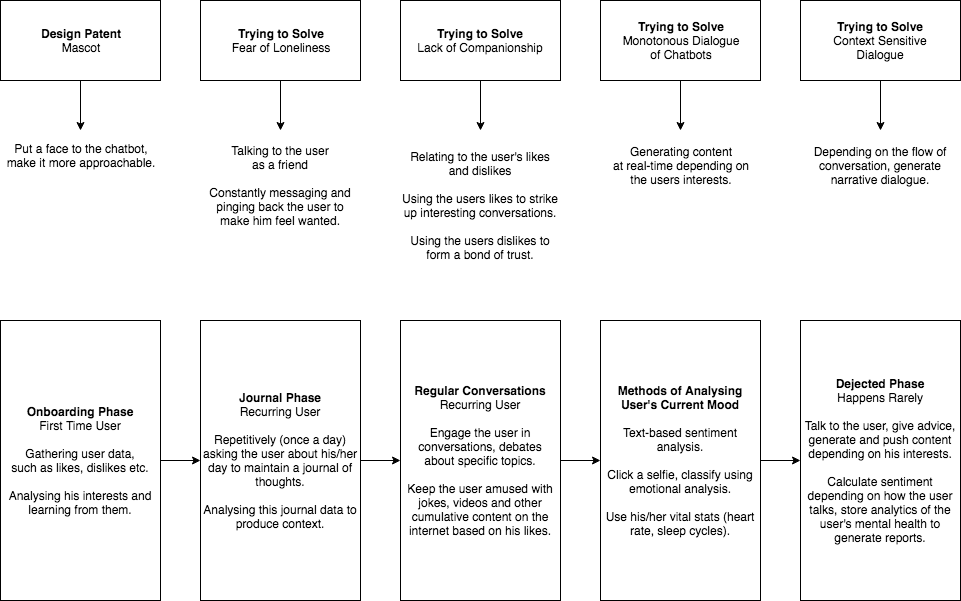
\includegraphics[width=6cm]{images/inventive-steps.png}
    \caption{Inventive Steps}
    \label{fig:inventive-steps}
\end{figure}

\subsubsection{Conversational Trees}

\begin{figure}[H]
    \centering
    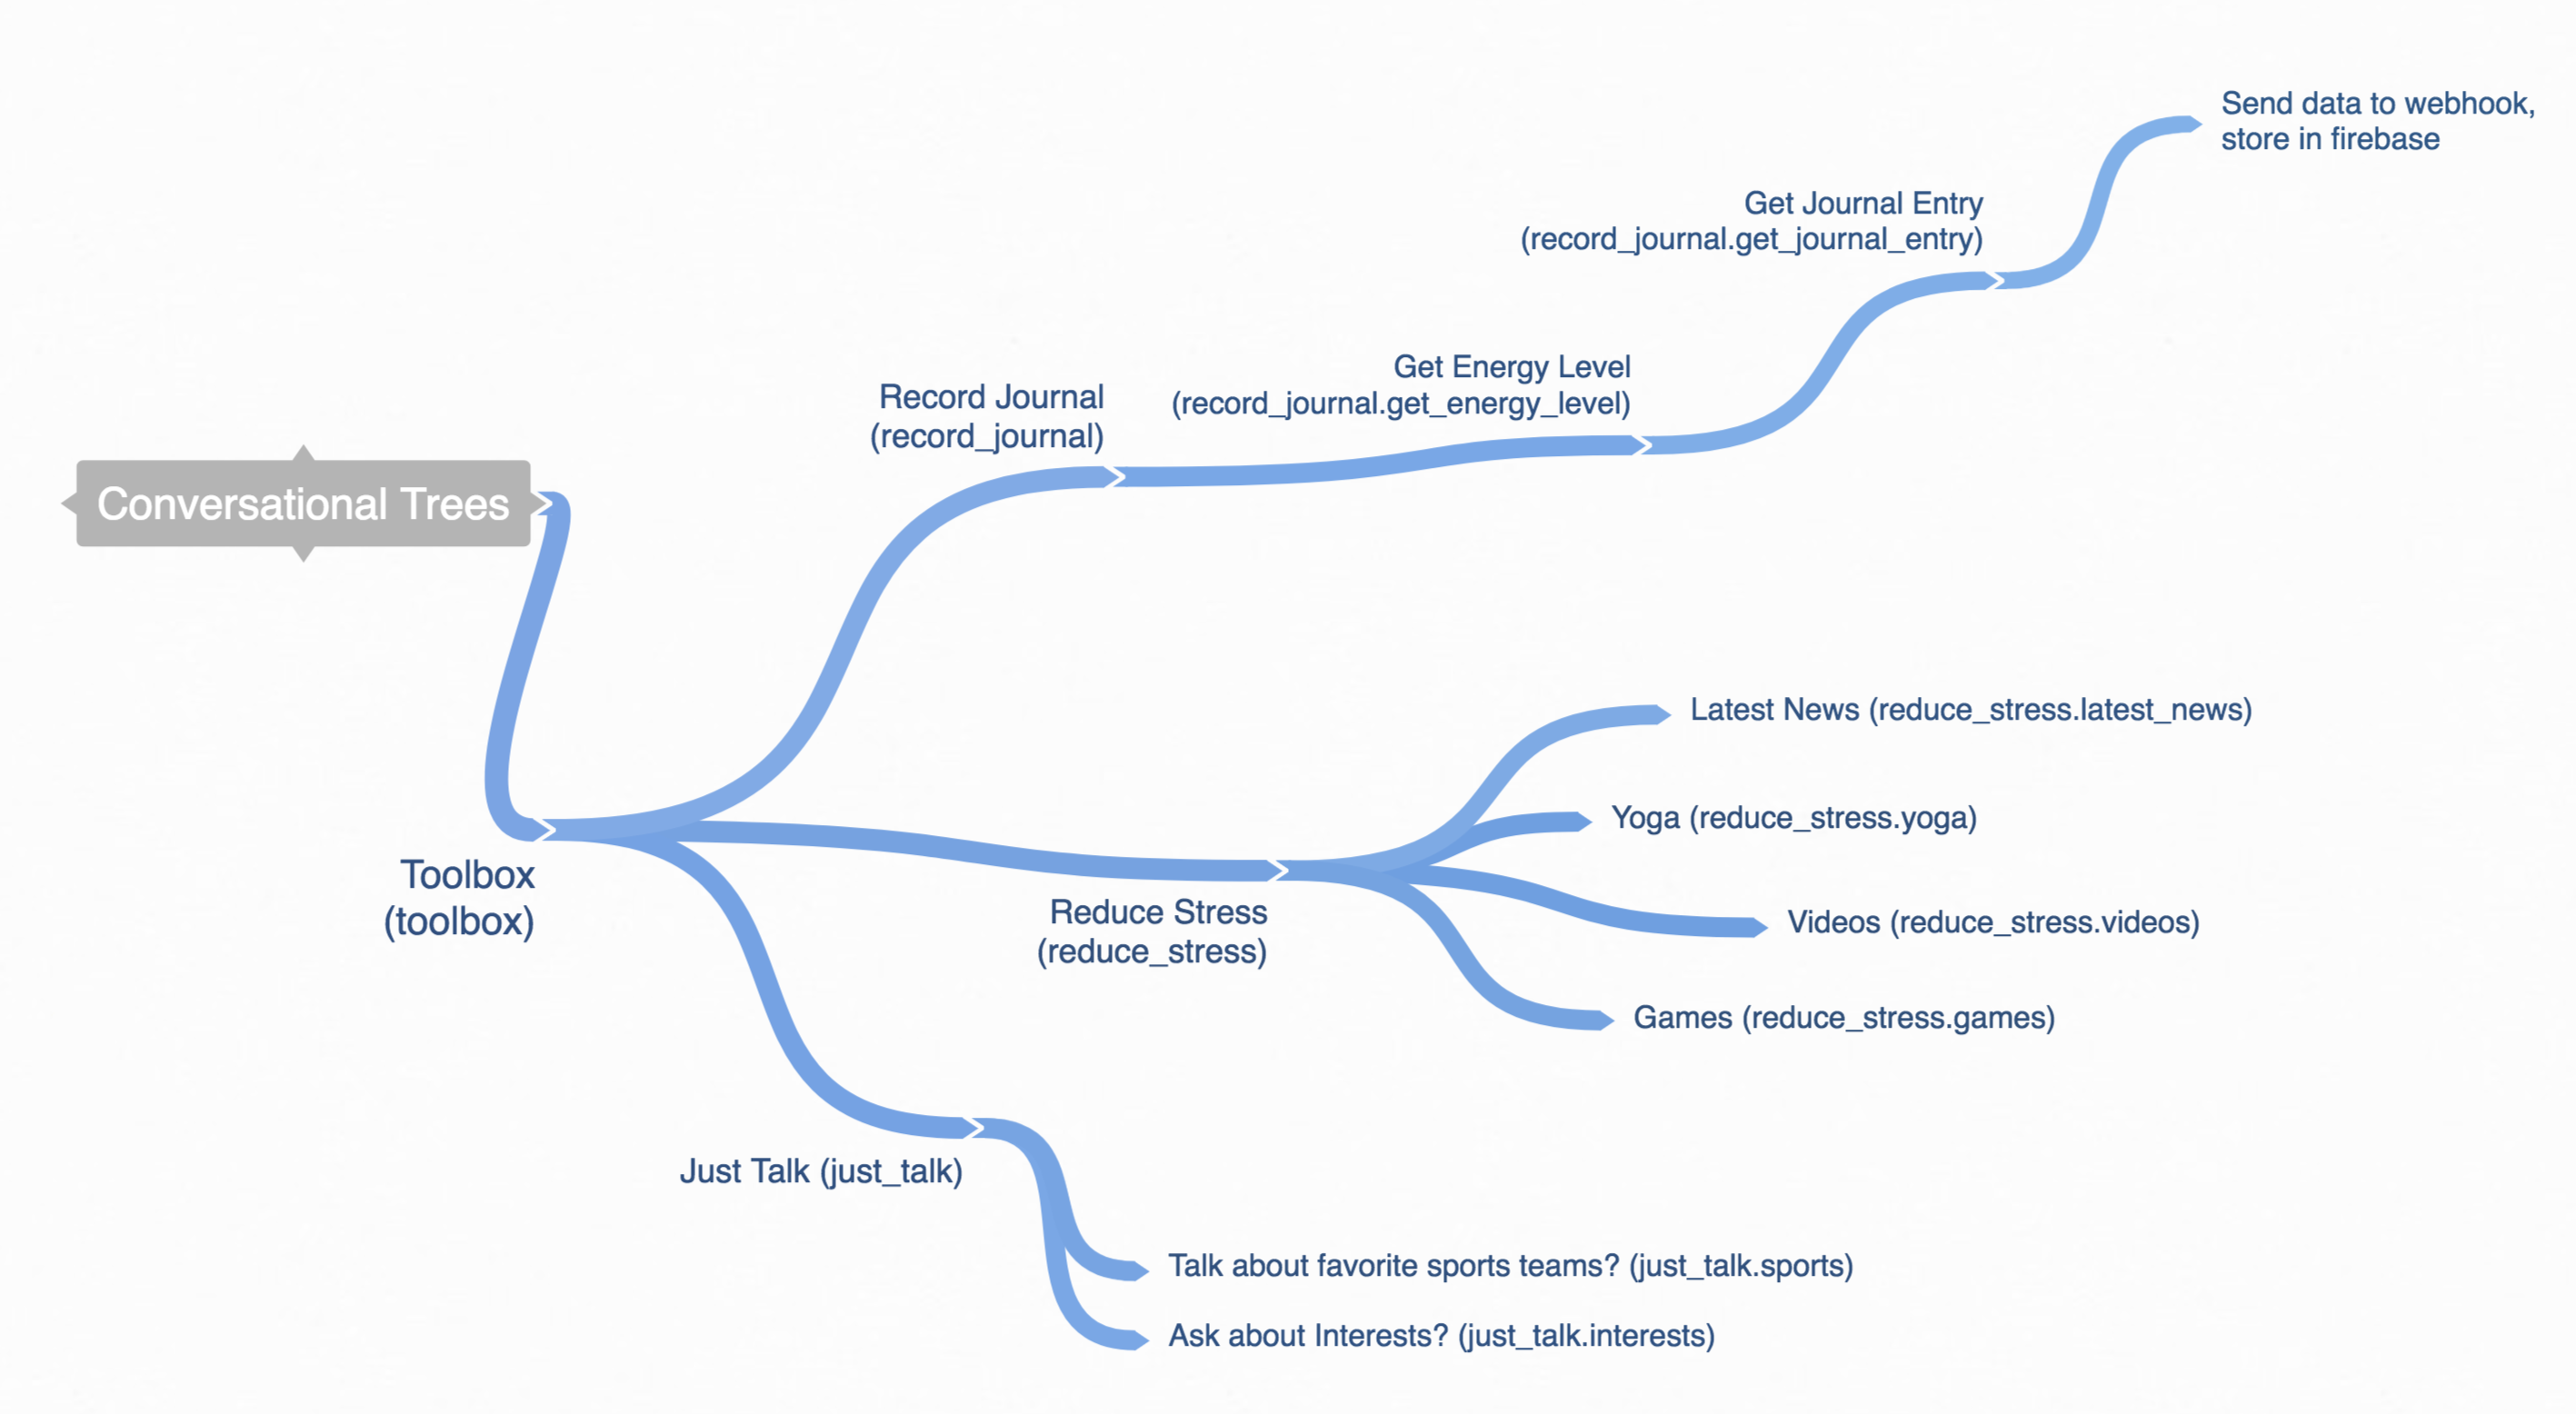
\includegraphics[width=6cm]{images/conversational-trees.png}
    \caption{Conversational Trees of the Chatbot}
    \label{fig:conversational-trees}
\end{figure}

\subsection{Sentiment Analysis Anatomy}

VADER (Valence Aware Dictionary and sEntiment Reasoner) is a model that is used to predict the sentiment type and sentiment score of a particular sentence or a word input. It gives out an accurate score of each of the three sentiments - positive, negative and neutral. The reason for the preference of this tool compared to any other machine learning approach is the surpassing the complexity of a voluminous dataset. VADER has a Dictionary of lexicons that are used to predict the score of the sentences.

\begin{figure}[H]
    \centering
    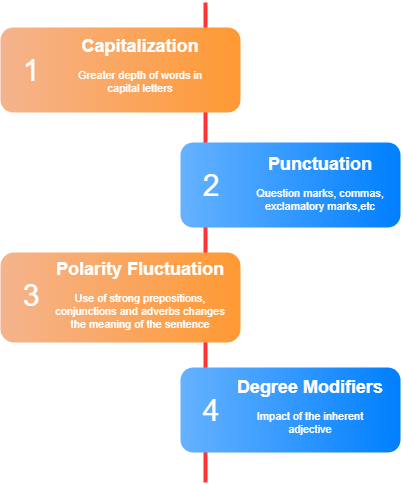
\includegraphics[width=6cm]{images/vader-model.png}
    \caption{Steps of the VADER Model}
    \label{fig:vader-model}
\end{figure}

\subsection{Word2Vec (NLP) Structure}

Word2vec is a two-layer neural net that processes text. Its input is a text corpus and its output is a set of vectors: feature vectors for words in that corpus. While Word2vec is not a deep neural network, it turns text into a numerical form that deep nets can understand. Deeplearning4j implements a distributed form of Word2vec for Java and Scala, which works on Spark with GPUs. Word2vec’s applications extend beyond parsing sentences in the wild. It can be applied just as well to genes, code, likes, playlists, social media graphs and other verbal or symbolic series in which patterns may be discerned.

\begin{figure}[H]
    \centering
    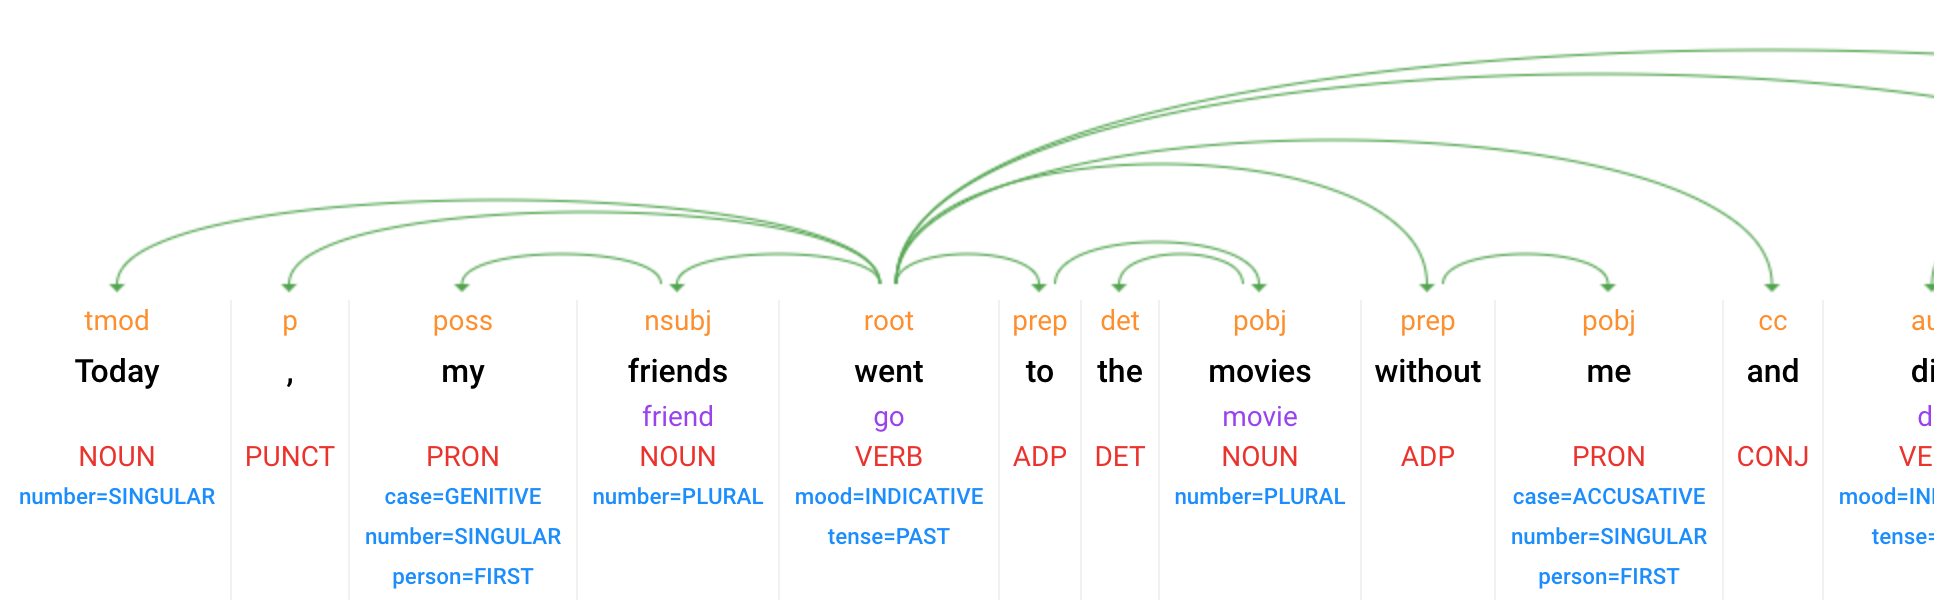
\includegraphics[width=6cm]{images/syntax-parsing.png}
    \caption{Syntax Parsing and Breakdown to Parts of Speech}
    \label{fig:syntax-parsing}
\end{figure}

Why? Because words are simply discrete states like the other data mentioned above, and we are simply looking for the transitional probabilities between those states: the likelihood that they will co-occur. So gene2vec, like2vec and follower2vec are all possible. With that in mind, the tutorial below will help you understand how to create neural embeddings for any group of discrete and co-occurring states. The purpose and usefulness of Word2vec is to group the vectors of similar words together in vectorspace. That is, it detects similarities mathematically. Word2vec creates vectors that are distributed numerical representations of word features, features such as the context of individual words. It does so without human intervention.

\begin{figure}[H]
    \centering
    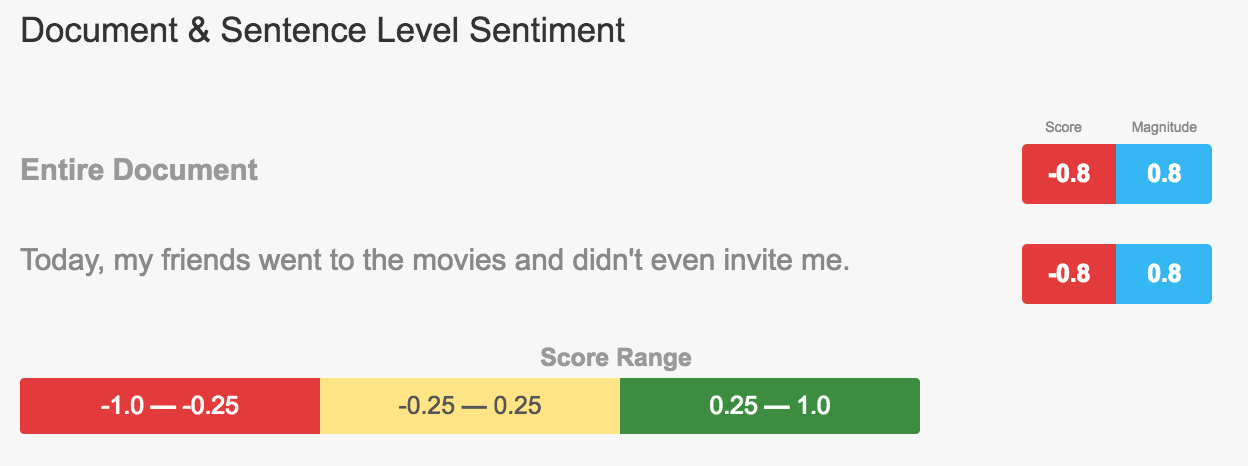
\includegraphics[width=6cm]{images/sentiment-analysis.png}
    \caption{Sentiment Analysis Response}
    \label{fig:sentiment-analysis}
\end{figure}

Given enough data, usage and contexts, Word2vec can make highly accurate guesses about a word’s meaning based on past appearances. Those guesses can be used to establish a word’s association with other words (e.g. “man” is to “boy” what “woman” is to “girl”), or cluster documents and classify them by topic. Those clusters can form the basis of search, sentiment analysis and recommendations in such diverse fields as scientific research, legal discovery, e-commerce and customer relationship management. The output of the Word2vec neural net is a vocabulary in which each item has a vector attached to it, which can be fed into a deep-learning net or simply queried to detect relationships between words.

% Implementation

\section{Implementation}

\subsection{Hardware Applications}

Since this project and study was purely an algorithmic implementation and product engineering showcase, the hardware required is extremely minimal and found in abundance with most consumers. All the project requires is a Windows/Mac/Linux PC that has minimum system hardware requirements to build the source, and an Android/iOS device with Google Assistant or Facebook Messenger installed to be able to test and run the application.

\subsection{Software Applications}

\begin{itemize}
    \item Operating System: Mac, Linux, Windows 8/10
    \item Programming Languages: Python, Node.js
    \item Chatbot Framework: DialogFlow
    \item Deep Learning Framework: Tensorflow
    \item Editors: Visual Studio Code, Jupyter Notebook
    \item Server: Heroku
\end{itemize}

\subsection{Procedure}

This subsection extensively talks about the artificial intelligence involved in our project.

\subsubsection{Project File Structure}

Organizing files on your computer is just like organizing anything else. Say you want to organize your clothes. You might sort each type of clothes into separate stacks. Then you might pair the socks or group all the shirts by color. Or, you could throw everything into one drawer and hope you can find the right pair of socks when you need it. And that's how we typically treat our files: we save files randomly to our Desktop and Documents folders, then waste time searching for files every day.

\begin{figure}[H]
    \centering
    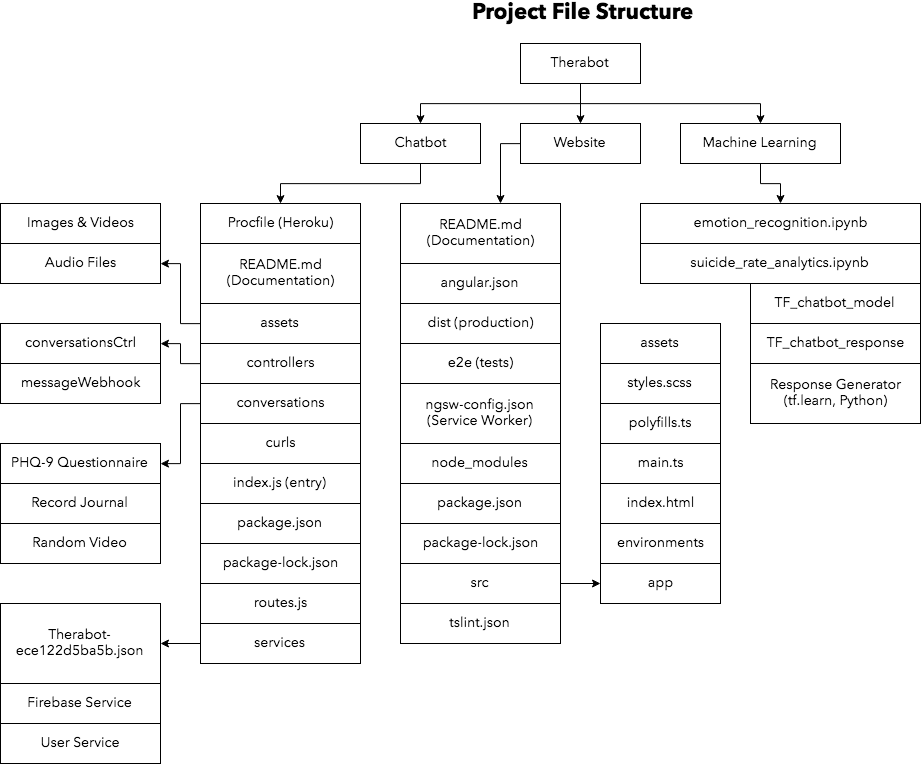
\includegraphics[width=6cm]{images/project-file-structure.png}
    \caption{Project File Structure}
\end{figure}

Folder structures can help, just like drawers and dividers can keep your clothes organized. A folder structure is the way folders are organized on your computer. As folders are added over time, you can either keep them at the same level—like Folders 1, 2, and 3 in the chart below—or nest them within each other for a hierarchy—like Subfolders 1B and 1B-1 below. Nested folders generally make it easier to find specific files later, because you don’t have to sift through all your files at once.

\subsubsection{Dataset Collection}

Our project requires an enormous amount of data in the form of conversational corpus. We have created a simple dataset in the form of questions and answers that would enable our tensorflow model to train with the generated responses. In order to incorporate the power of crowdsourcing, we have created a Google Form that would enable the community to facilitate wide range of responses.

\begin{figure}[H]
    \centering
    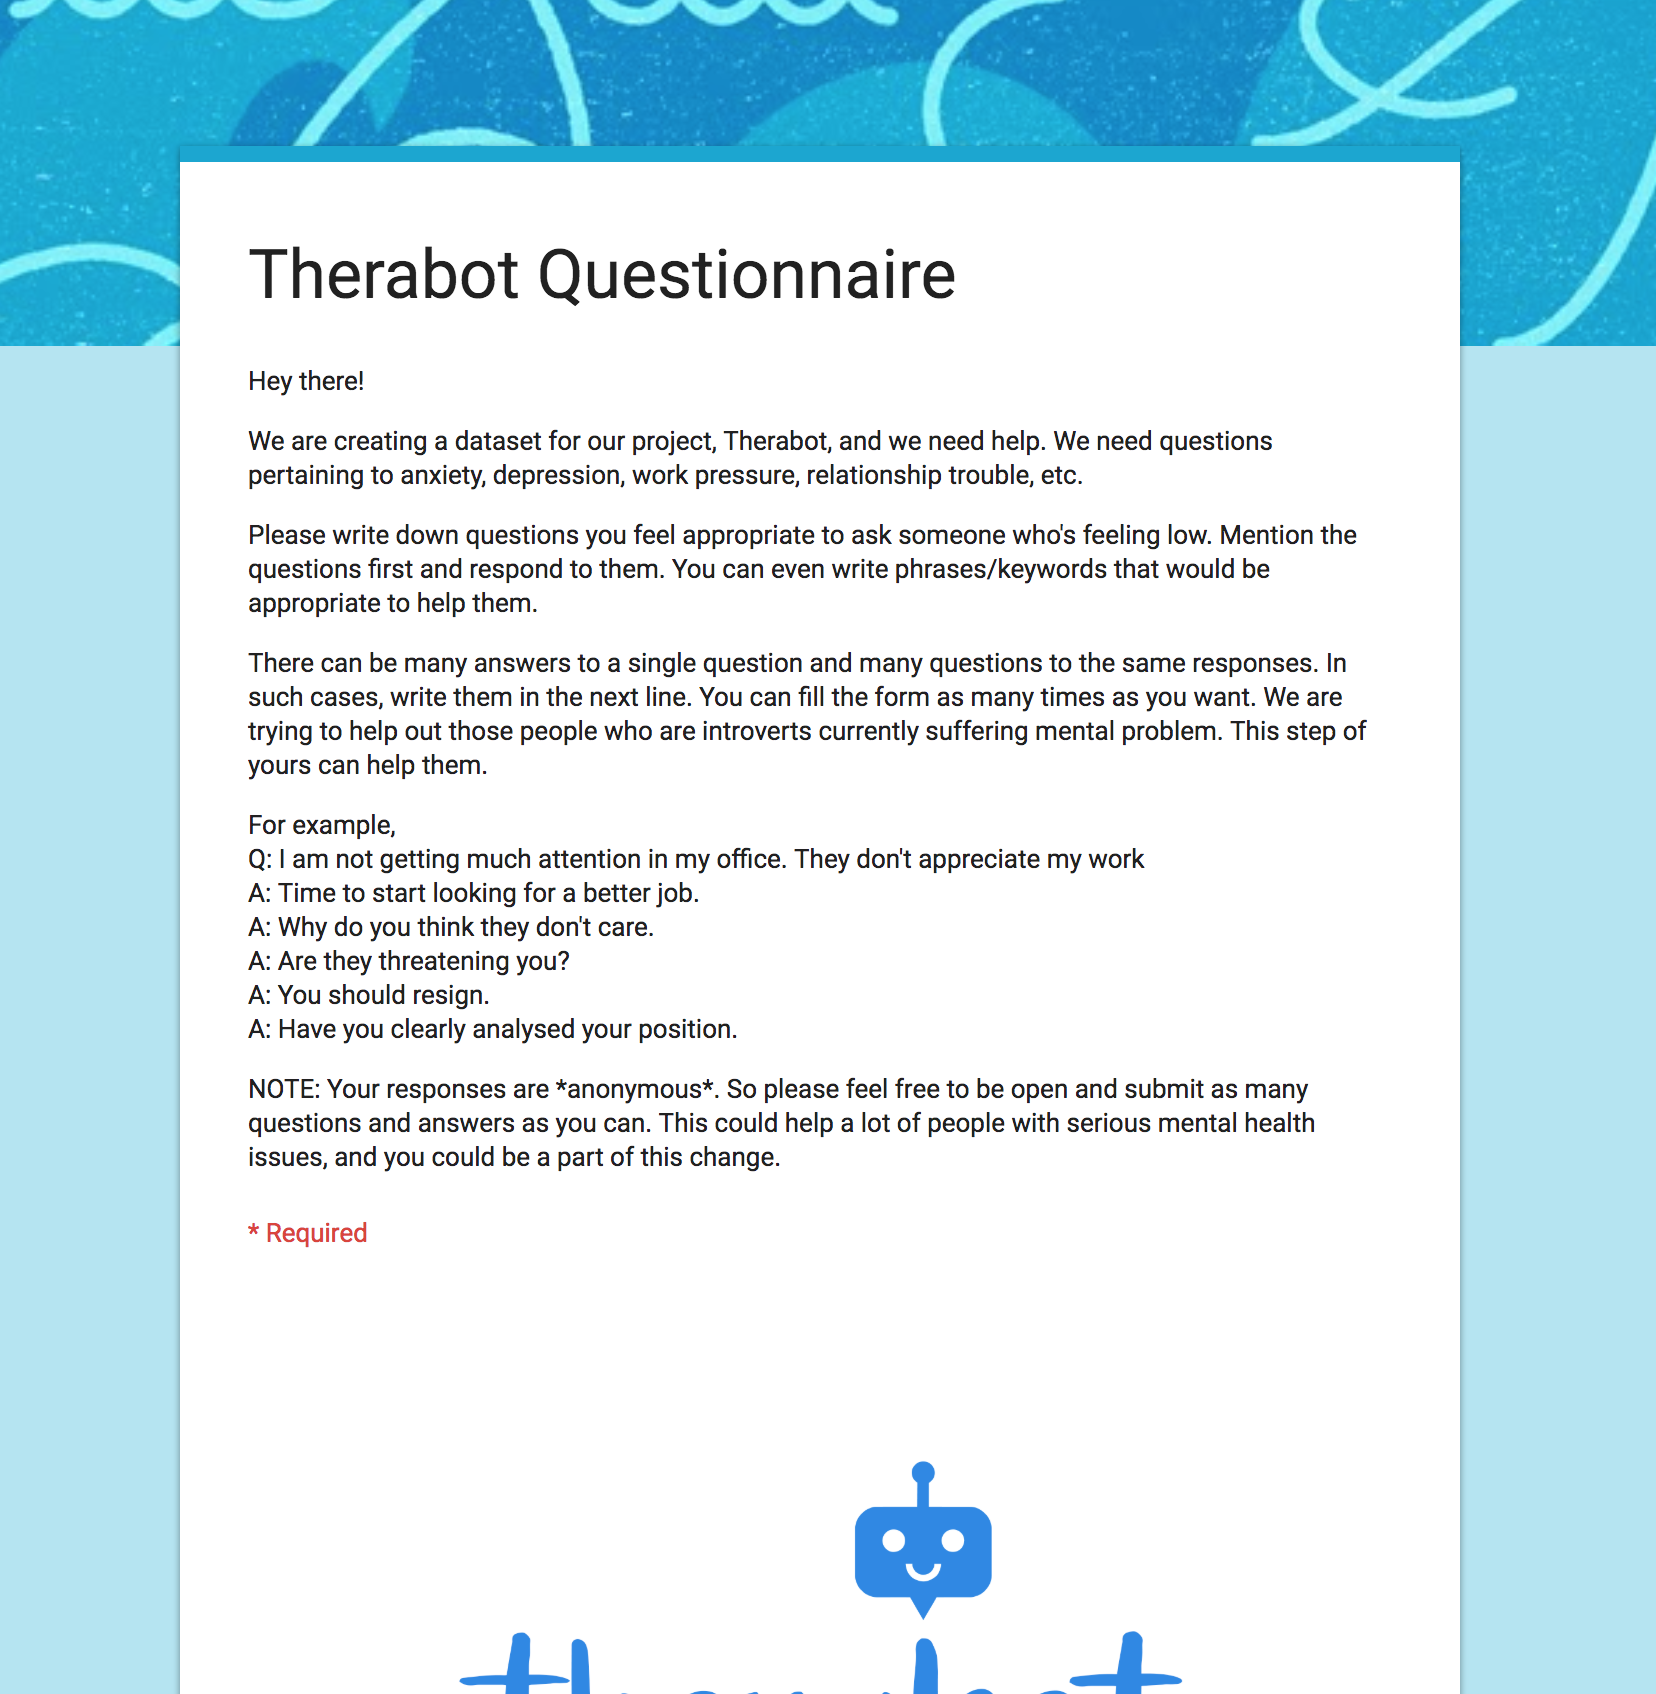
\includegraphics[width=6cm]{images/therabot-questionnaire.png}
    \caption{Therabot Questionnaire}
\end{figure}

We’ve also referred the Facebook Data Corpus and Cornell Movie Corpus for understanding the structure of data and scraped various datasets on Kaggle cherrypicking the from various conversational models to statistical data.

\subsubsection{Setting up the Environment}

We’ll need to download the Natural Language Processing Library as well as Tensorflow for higher order numerical computation.

\textbf{Installing NLTK:}
For Windows, Linux and Mac users we recommend installing Anaconda over which the NLP library can be set up. The following command will automatically fetch all the resources and install the Natural Language Toolkit.


\texttt{sudo pip install -U nltk}

\textbf{Installing TensorFlow:}
An environment must be created in in which TensorFlow will be installed. All the necessary pre-requisites and a step-by-step guide to a successful installation are available at https://www.tensorflow.org/install/.

\subsubsection{Data Preprocessing}

The accumulated dataset is subjected to a lot of functions which optimize its use during training. This cleaning process is what constitutes the preprocessing.

\paragraph{Tokenizing}
The dataset contains paragraphs of sentences and well as individual sentences. In some cases, it is necessary to retrieve the sentence as a whole and sometimes as individual words. To facilitate this, the NLTK library has two predefined functions: \texttt{sent\_tokenize} and \texttt{word\_tokenize}.

\begin{figure}[H]
    \centering
    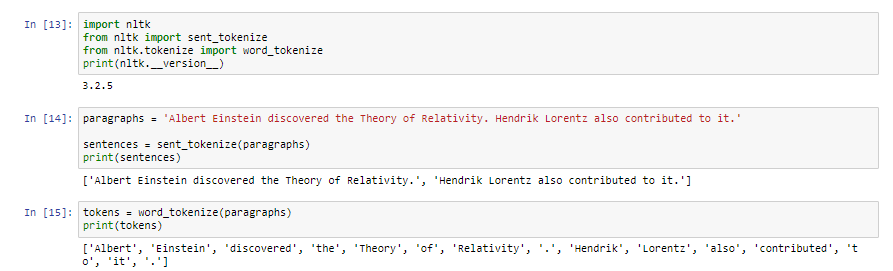
\includegraphics[width=6cm]{images/jupyter-notebook-tokenizing.png}
    \caption{Jupyter Notebook - Tokenizing}
\end{figure}

Similarly, punctuation and stop words can also be filtered out.

\paragraph{Stemming}
While storing the user’s data into Firebase, we need to peddle down the words in these sentences to their purest form or root. This process is called stemming.

\begin{figure}[H]
    \centering
    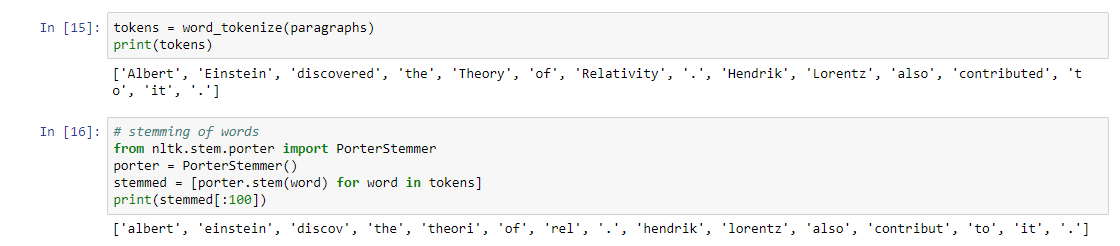
\includegraphics[width=6cm]{images/jupyter-notebook-stemming.png}
    \caption{Jupyter Notebook - Stemming}
\end{figure}

\subsection{Algorithms}

\subsubsection{Linear Regression}

When we have a single in put attribute $(x)$ and we want to use linear regression, this is called \textbf{Simple Linear Regression}.

With simple linear regression we want to model our data as follows:
\[
    y = B_{0} + B_{1} * x
\]

This is a line where $y$ is the output variable we want to predict, $x$ is the input variable we know and $B_{0}$ and $B_{1}$ are coefficients we need to estimate.

$B_{0}$ is called the intercept because it determines where the line intercepts the $y$ axis. In machine learning we can call this the bias, because it is added to offset all predictions that we make. The $B_{1}$ term is called the slope because it defines the slope of the line or how $x$ translates into a $y$ value before we add our bias.

The model is called Simple Linear Regression because there is only one input variable $(x)$. If there were more input variables (e.g. $x_{1}, x_{2}$, etc.) then this would be called Multiple Regression.

\subsubsection{Gradient Descent}

\textbf{Optimization} refers to the task of minimizing/maximizing an objective function $f(x)$ parameterized by $x$. In machine/deep learning terminology, it’s the task of minimizing the cost/loss function $J(w)$ parameterized by the model’s parameters $w$ \epsilon $R^d$.

Optimization algorithms (in case of minimization) have one of the following goals:
\begin{itemize}
    \item Find the global minimum of the objective function. This is feasible if the objective function is convex, i.e. any local minimum is a global minimum.
    \item Find the lowest possible value of the objective function within its neighborhood. That’s usually the case if the objective function is not convex as the case in most deep learning problems.
\end{itemize}

\textbf{Gradient Descent} is the most common optimization algorithm in machine learning and deep learning. It is a first-order optimization algorithm. This means it only takes into account the first derivative when performing the updates on the parameters. On each iteration, we update the parameters in the opposite direction of the gradient of the objective function $J(w)$ w.r.t the parameters where the gradient gives the direction of the steepest ascent. The size of the step we take on each iteration to reach the local minimum is determined by the learning rate $α$. Therefore, we follow the direction of the slope downhill until we reach a local minimum.

\begin{figure}[H]
    \centering
    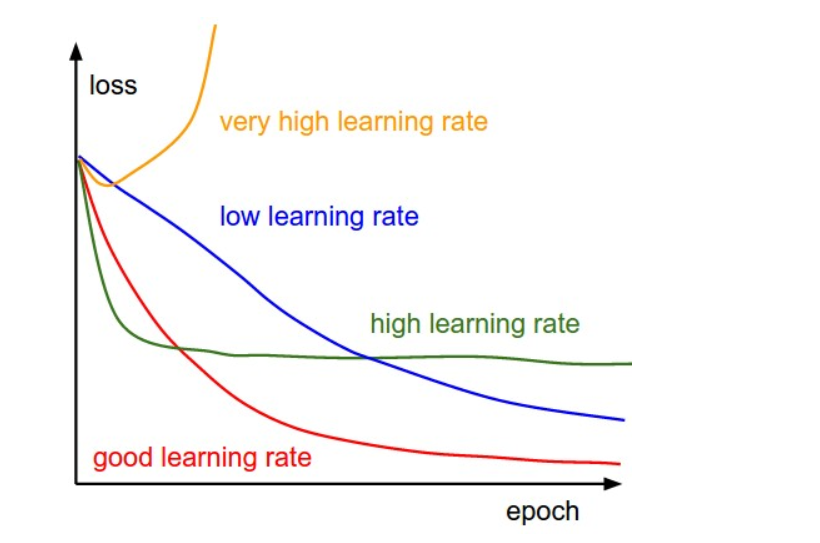
\includegraphics[width=6cm]{images/gradient-descent-different-learning-rates.png}
    \caption{Gradient Descent with Different Learning Rates}
\end{figure}

\[
    \frac{\delta}{\delta m} = \frac{2}{N} \sum_{i=1}^{N} - x_{i}(y_{i} - (mx_{i} +b))
\]

The coefficients used in simple linear regression can be found using stochastic gradient descent. Linear regression is a linear system and the coefficients can be calculated analytically using linear algebra. Stochastic gradient descent is not used to calculate the coefficients for linear regression in practice (in most cases). Linear regression does provide a useful exercise for learning stochastic gradient descent which is an important algorithm used for minimizing cost functions by machine learning algorithms.

\begin{center}
\begin{tabular}{|c|c|}
    \hline
    $B_{0}$ & $B_{1}$ \\ [0.5ex]
    \hline
    0.01 & 0.01 \\
    \hline
    0.0397 & 0.0694 \\
    \hline
    0.066527 & 0.176708 \\
    \hline
    0.08056049 & 0.21880847 \\
    \hline
    0.1188144616 & 0.410078328 \\
    \hline
    0.1235255337 & 0.4147894001 \\
    \hline
    0.1439944904 & 0.4557273134 \\
    \hline
    0.1543254529 & 0.4970511637 \\
    \hline
    0.1578706635 & 0.5076867953 \\
    \hline
    0.1809076171 & 0.6228715633 \\
    \hline
\end{tabular}
\end{center}

About 10 iterations or 2 epochs is a nice round number and a good place to stop. You could keep going if you wanted. Your values should match closely, but may have minor differences. You can plug each pair of coefficients back into the simple linear regression equation. This is useful because we can calculate a prediction for each training instance and in turn calculate the error.

\subsubsection{Logistic Regression}

Logistic Regression is a classification algorithm. It is used to predict a binary outcome (1 / 0, Yes / No, True / False) given a set of independent variables. To represent binary / categorical outcome, we use dummy variables. You can also think of logistic regression as a special case of linear regression when the outcome variable is categorical, where we are using log of odds as dependent variable. In simple words, it predicts the probability of occurrence of an event by fitting data to a logit function.

The fundamental equation of generalized linear model is:
\[
    g(E(y)) = α + βx1 + γx2    
\]

Here, $g()$ is the link function, $E(y)$ is the expectation of target variable and $α + β_{x1} + γ_{x2}$ is the linear predictor ($α, β, γ$ to be predicted). The role of link function is to ‘link’ the expectation of $y$ to linear predictor.

On further deriving the equation, we get this:

\[
    log(\frac{p}{1 - p}) = \beta_{0} + \beta(Age)
\]

This is the equation used in Logistic Regression. Here $(\frac{p}{1-p})$ is the odd ratio. Whenever the log of odd ratio is found to be positive, the probability of success is always more than 50\%. A typical logistic model plot is shown below. You can see probability never goes below 0 and above 1.

\begin{figure}[H]
    \centering
    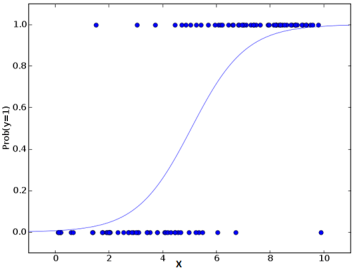
\includegraphics[width=6cm]{images/logistic-regression-plot.png}
    \caption{Typical Logistic Regression Model Plot}
\end{figure}

\subsubsection{Softmax Function}

Softmax function calculates the probabilities distribution of the event over ‘$n$’ different events. In general way of saying, this function will calculate the probabilities of each target class over all possible target classes. Later the calculated probabilities will be helpful for determining the target class for the given inputs.

\begin{figure}[H]
    \centering
    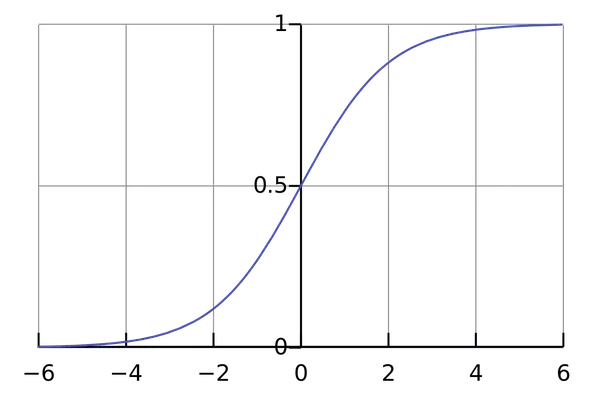
\includegraphics[width=6cm]{images/softmax-function.png}
    \caption{Softmax Function}
\end{figure}

The main advantage of using Softmax is the output probabilities range. The range will 0 to 1, and the sum of all the probabilities will be equal to one. If the softmax function used for multi-classification model it returns the probabilities of each class and the target class will have the high probability.

The formula computes the exponential ($e$-power) of the given input value and the sum of exponential values of all the values in the inputs. Then the ratio of the exponential of the input value and the sum of exponential values is the output of the softmax function.

\[
    P(y = j | z^{(i)}) = \phi_{softmax} (z^{(i)}) = \frac{e^z}{\sum_{j=1}^{k} e^z_k}
\]

\[
    z = w_0x_0 + w_1x_1 + ... + w_mx_m = \sum_{i=0}^{m} w_ix_i = w^Tx
\]

The softmax function is often used in the final layer of a neural network-based classifier. Such networks are commonly trained under a log loss (or cross-entropy) regime, giving a non-linear variant of multinomial logistic regression.

\subsection{Diagrams}

\subsubsection{Data Flow Diagram}

A Data Flow Diagram (DFD) is traditional visual representation of the information flows within a system. A neat and clear DFD can depict a good amount of the system requirements graphically. It can be manual, automated, or combination of both. It shows how information enters and leaves the system, what changes the information and where information is stored. The purpose of a DFD is to show the scope and boundaries of a system as a whole.

There are four major components or external agents involved in the system:
\begin{itemize}
    \item User
    \item DialogFlow Framework
    \item Machine Learning Model
    \item Firebase Database
\end{itemize}

\begin{figure}[H]
    \centering
    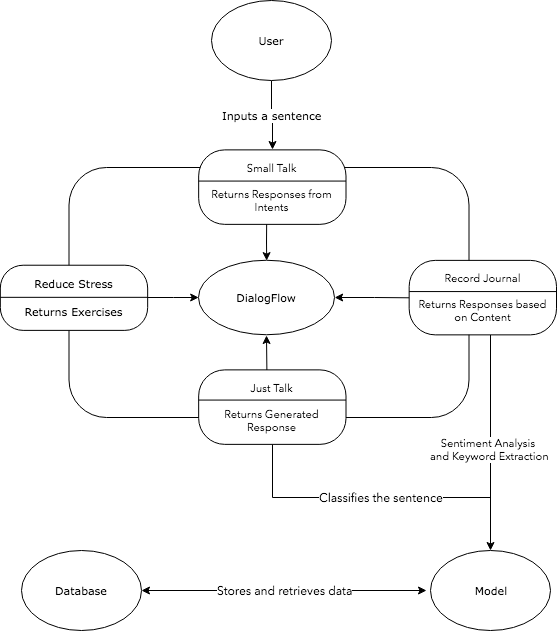
\includegraphics[width=6cm]{images/data-flow-diagram.png}
    \caption{Data Flow Diagram}
\end{figure}

\subsubsection{Sequence Diagram}

A sequence diagram shows object interactions arranged in time sequence. It depicts the objects and classes involved in the scenario and the sequence of messages exchanged between the objects needed to carry out the functionality of the scenario.

We have two different sequence diagrams here:
\begin{itemize}
    \item Onboarding Phase
    \item Regular Conversations
\end{itemize}

\begin{figure}[H]
    \centering
    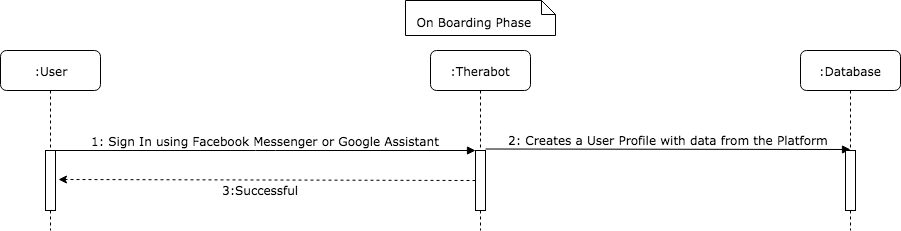
\includegraphics[width=6cm]{images/sequence-diagram-onboarding-phase.png}
    \caption{Sequence Diagram - Onboarding Phase}
\end{figure}

\begin{figure}[H]
    \centering
    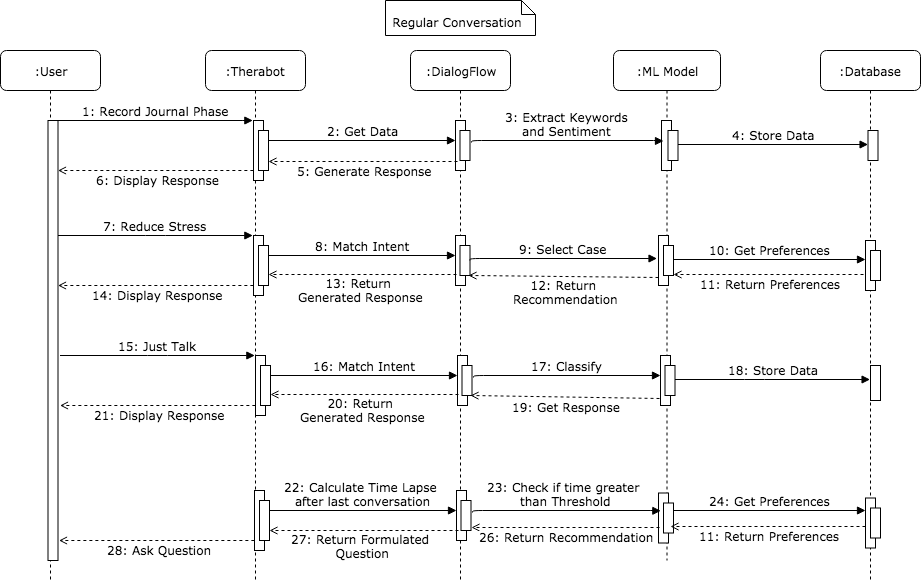
\includegraphics[width=6cm]{images/sequence-diagram-regular-conversations.png}
    \caption{Sequence Diagram - Regular Conversations}
\end{figure}

% Experimentation and Results

\section{Experimentation and Results}

\subsection{Screenshots}

\subsubsection{Website}

\noindent
Below are some screenshots of the website, which is hosted on the cloud. It is a Progressive Web App (PWA), meaning it can function as a functioning native Android/iOS application or a desktop web application on the same code.

\begin{figure}[H]
    \centering
    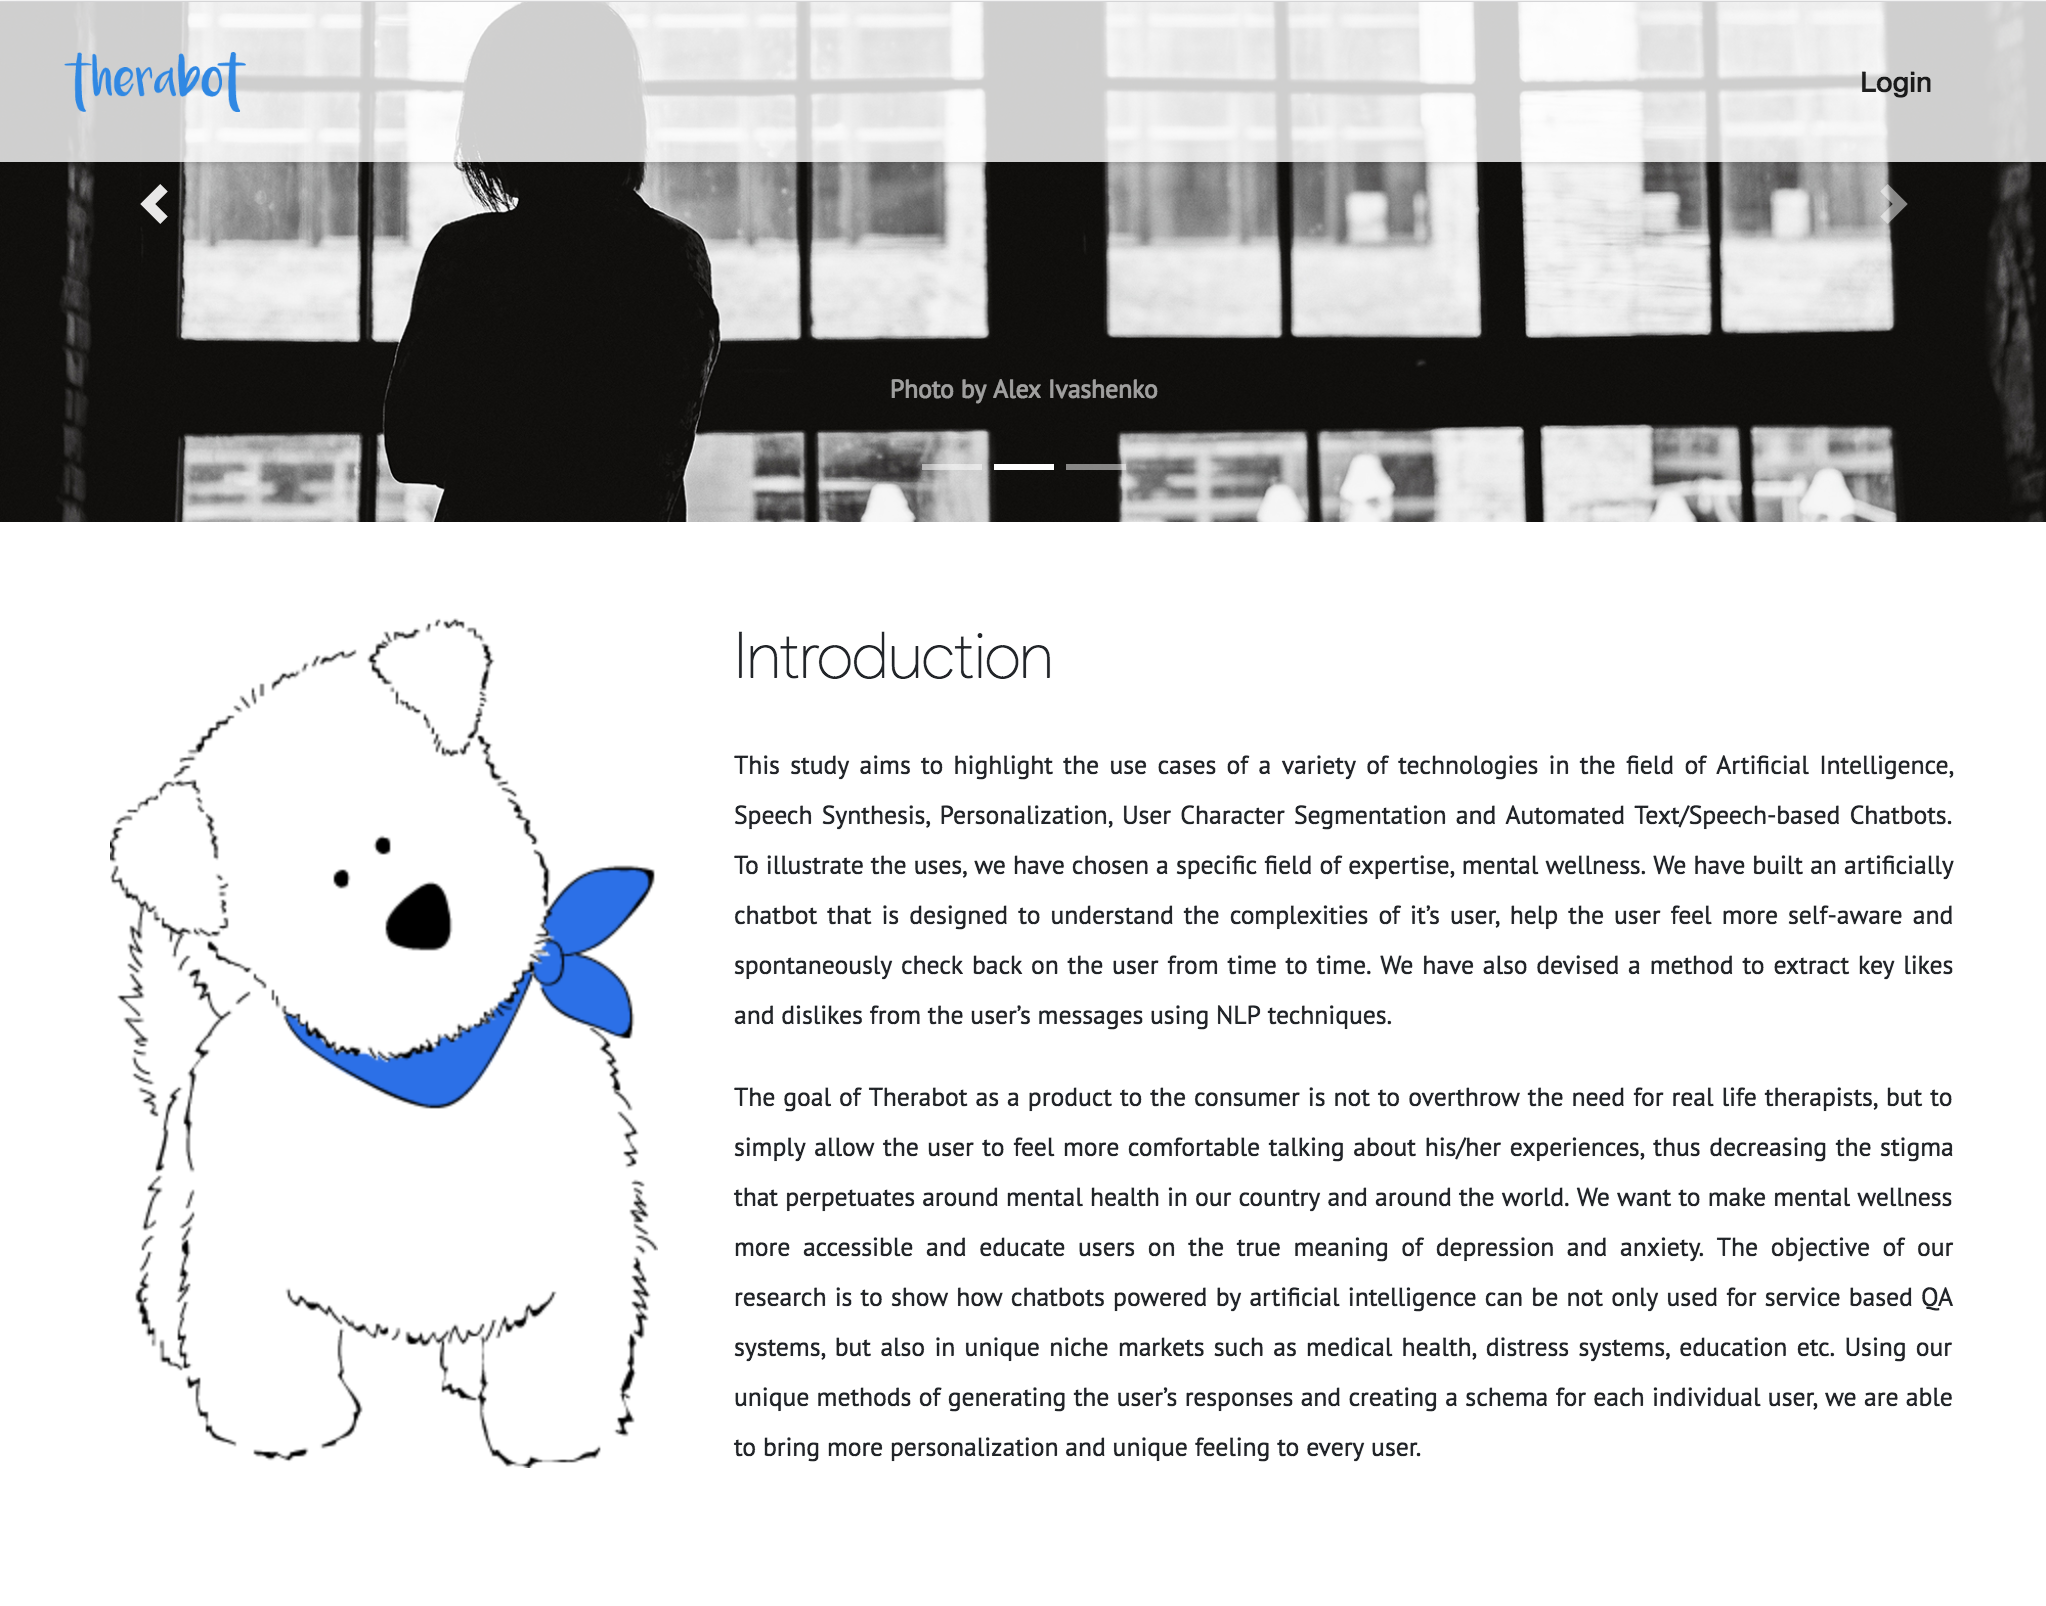
\includegraphics[width=6cm]{images/screenshots/website/website-introduction.png}
    \caption{Introduction}
\end{figure}

\begin{figure}[H]
    \centering
    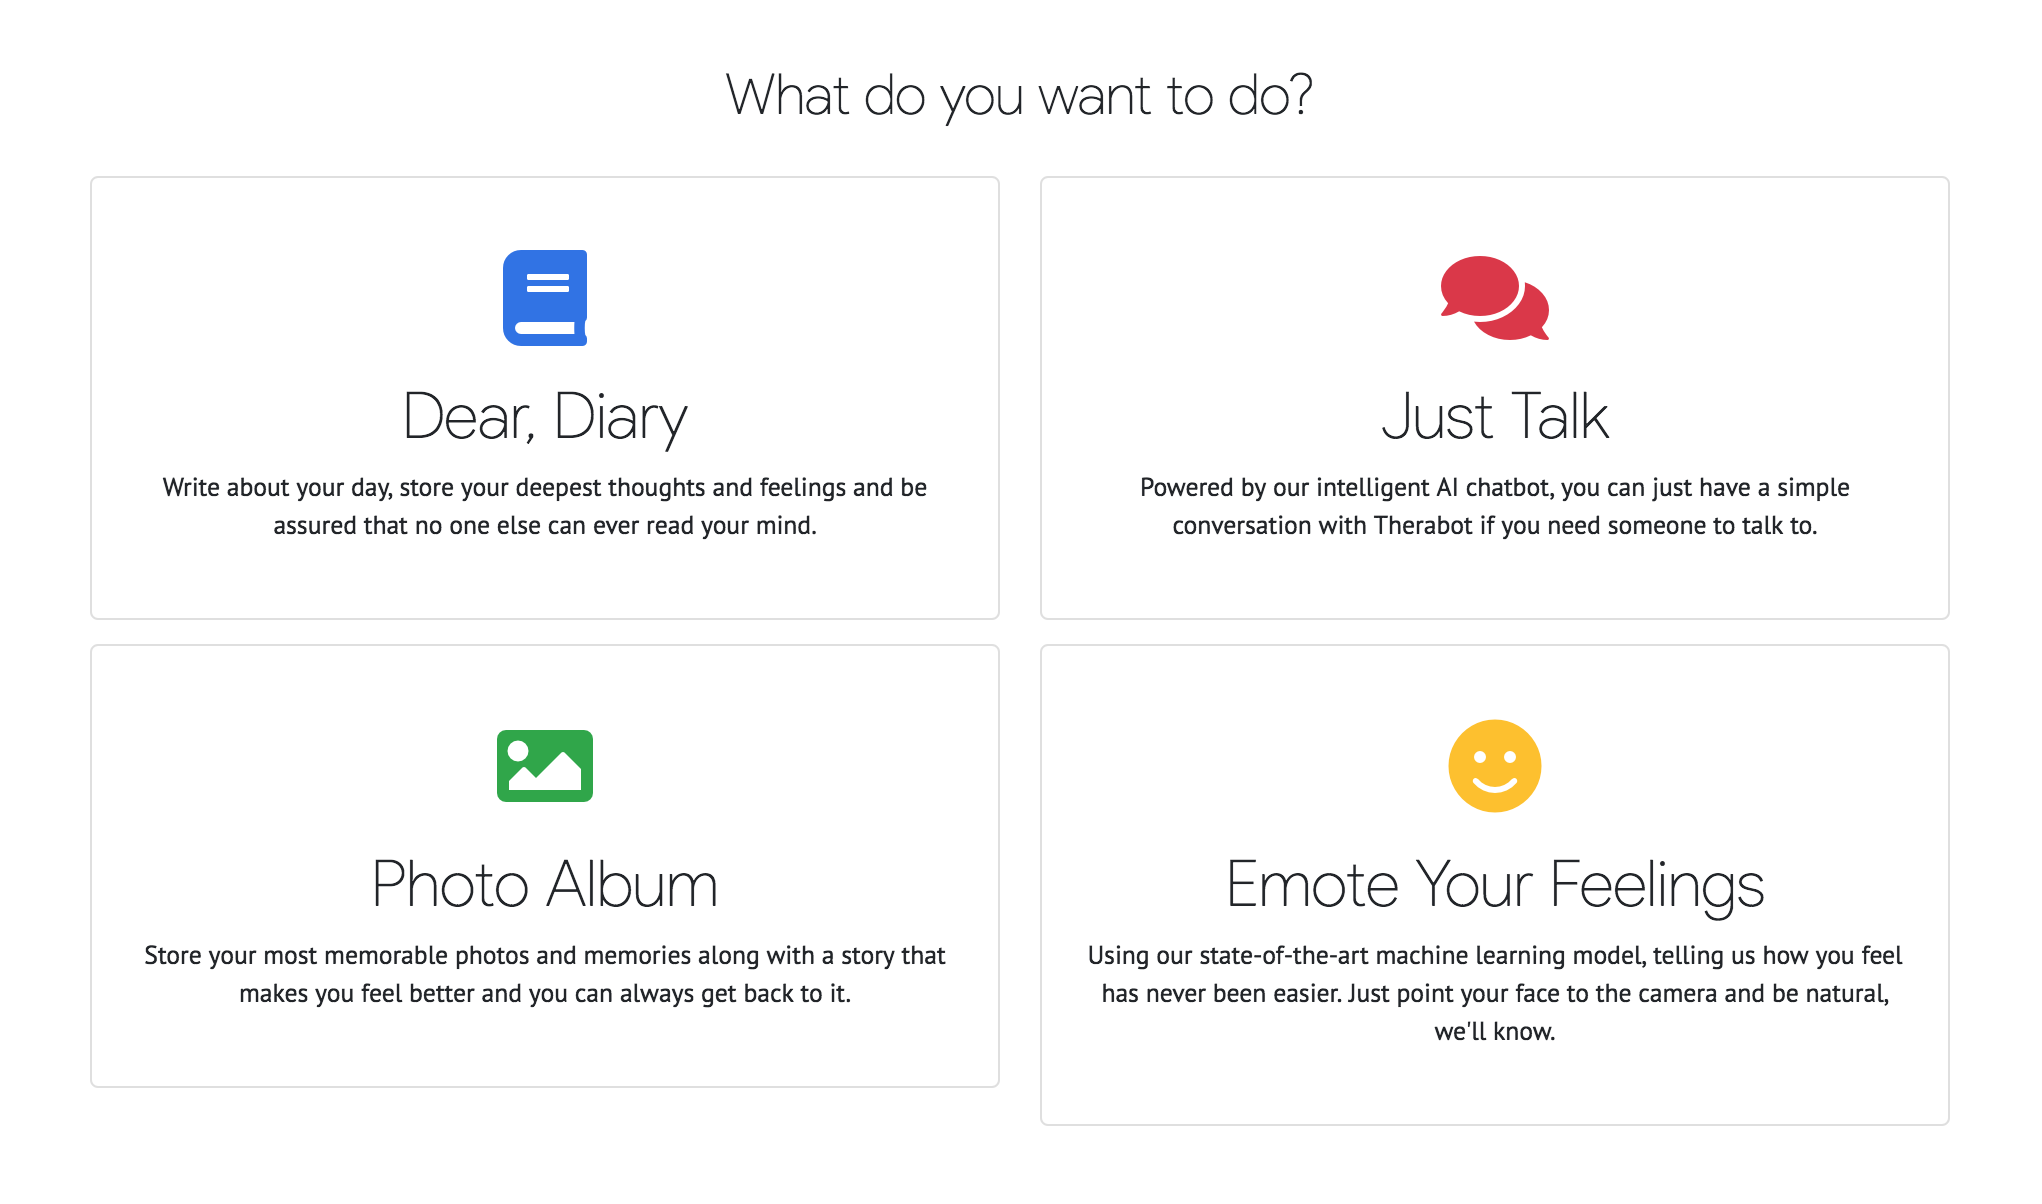
\includegraphics[width=6cm]{images/screenshots/website/website-modules.png}
    \caption{Modules on the Website}
\end{figure}

\begin{figure}[H]
    \centering
    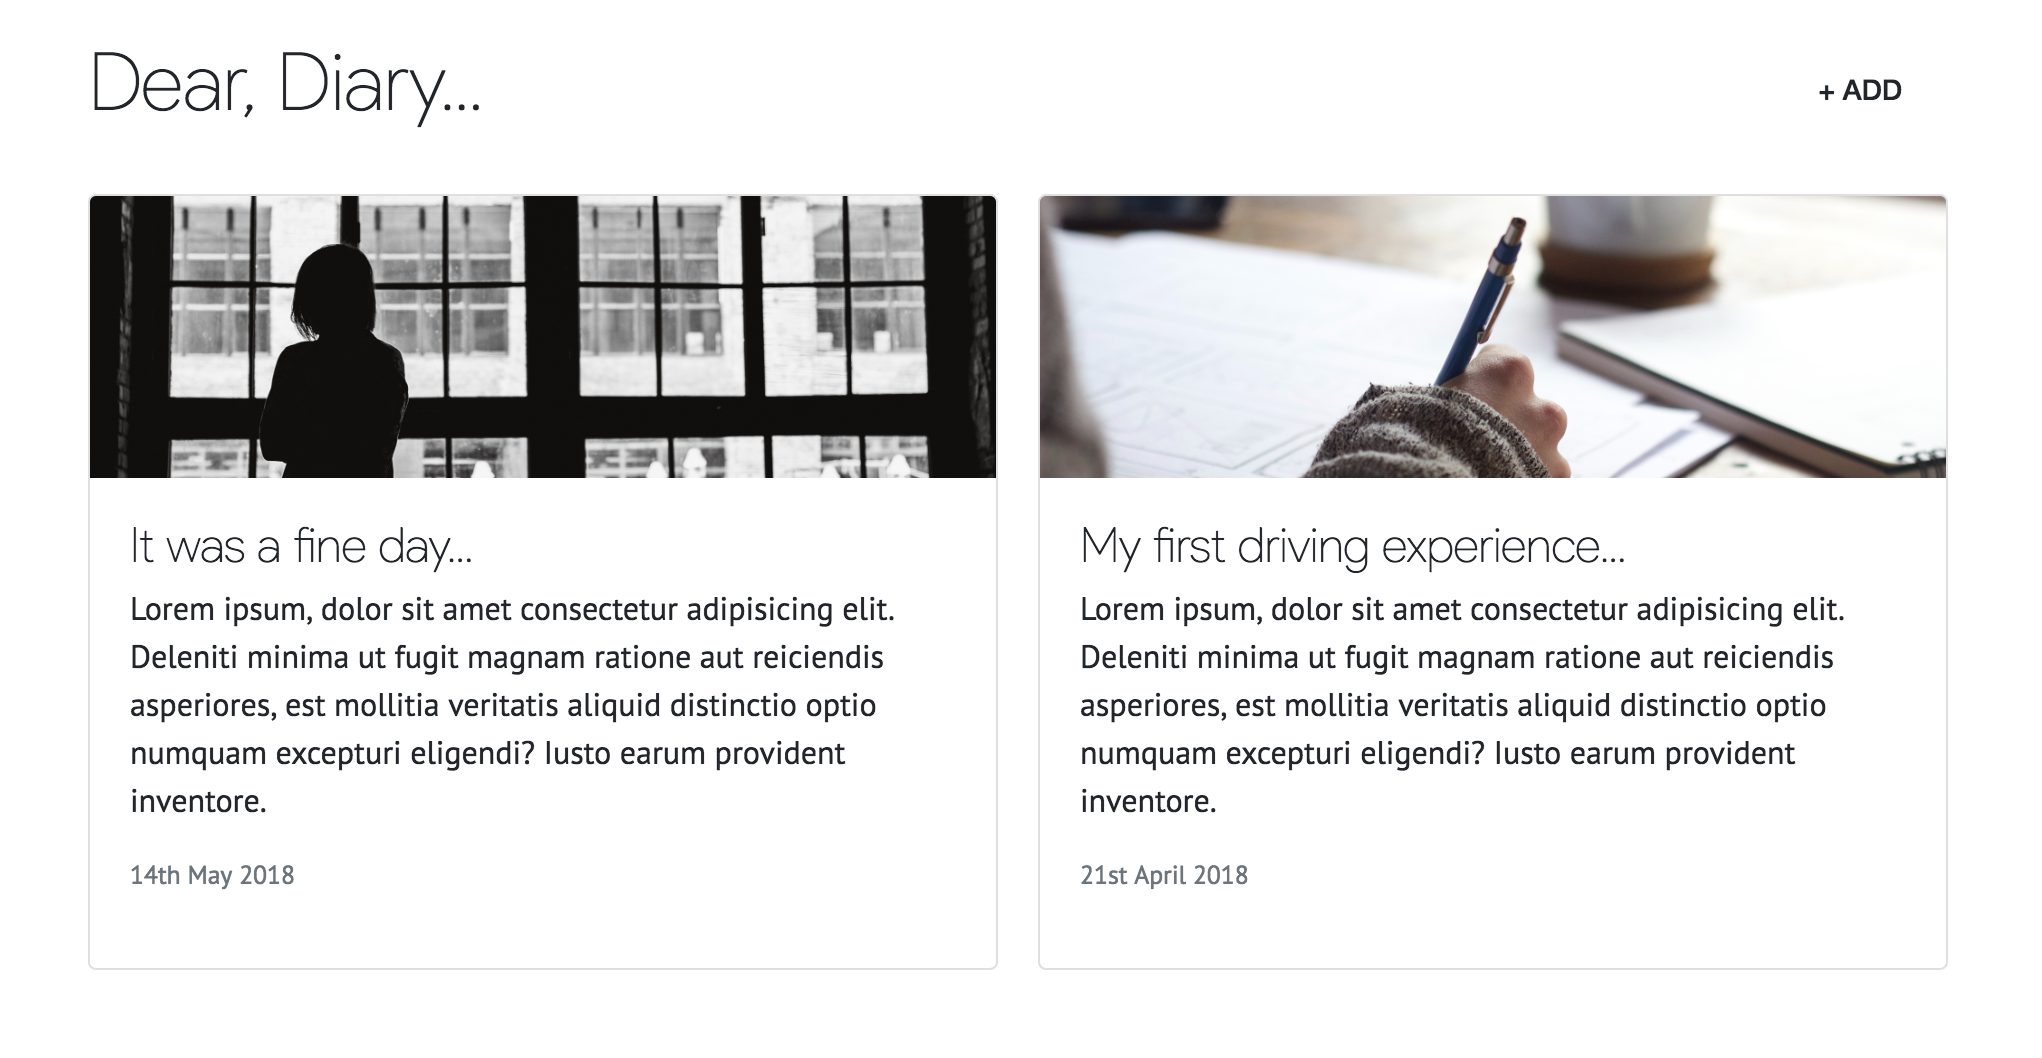
\includegraphics[width=6cm]{images/screenshots/website/website-dear-diary.png}
    \caption{Module \#1 - Dear Diary}
\end{figure}

\begin{figure}[H]
    \centering
    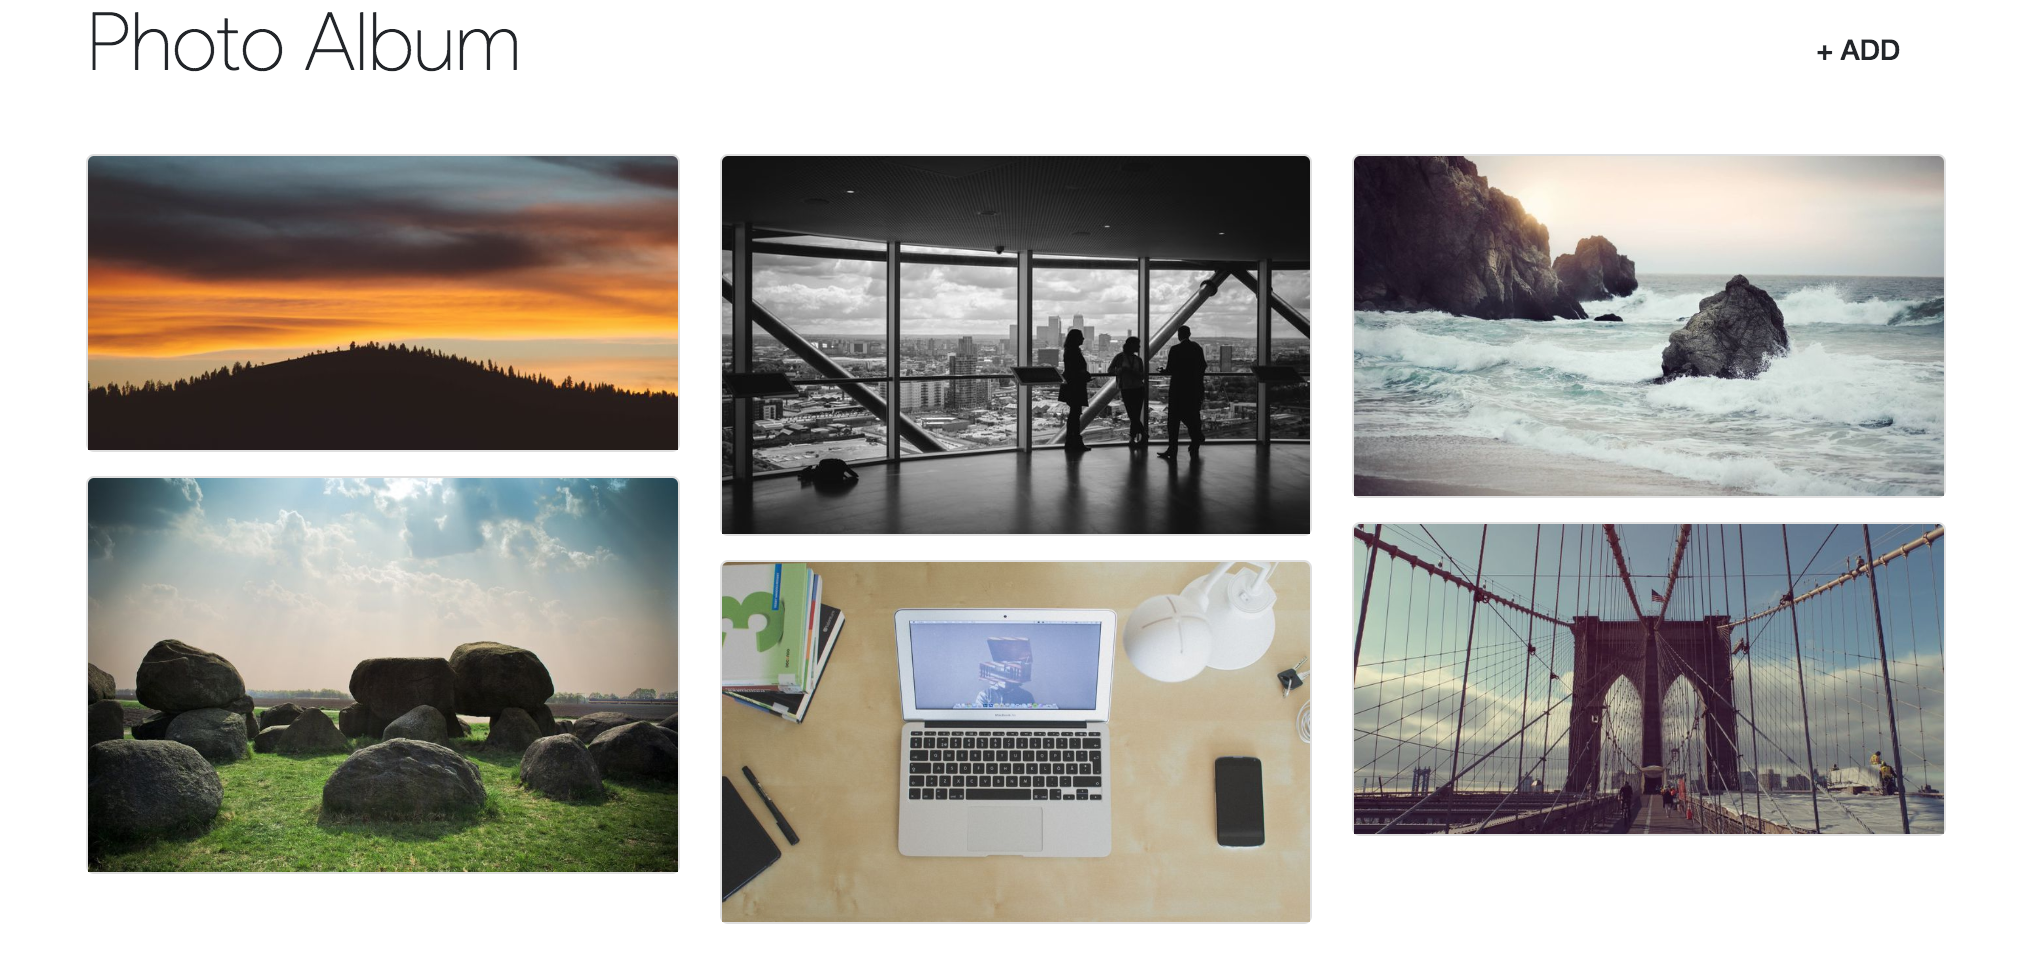
\includegraphics[width=6cm]{images/screenshots/website/website-photo-album.png}
    \caption{Module \#2 - Photo Album}
\end{figure}

\begin{figure}[H]
    \centering
    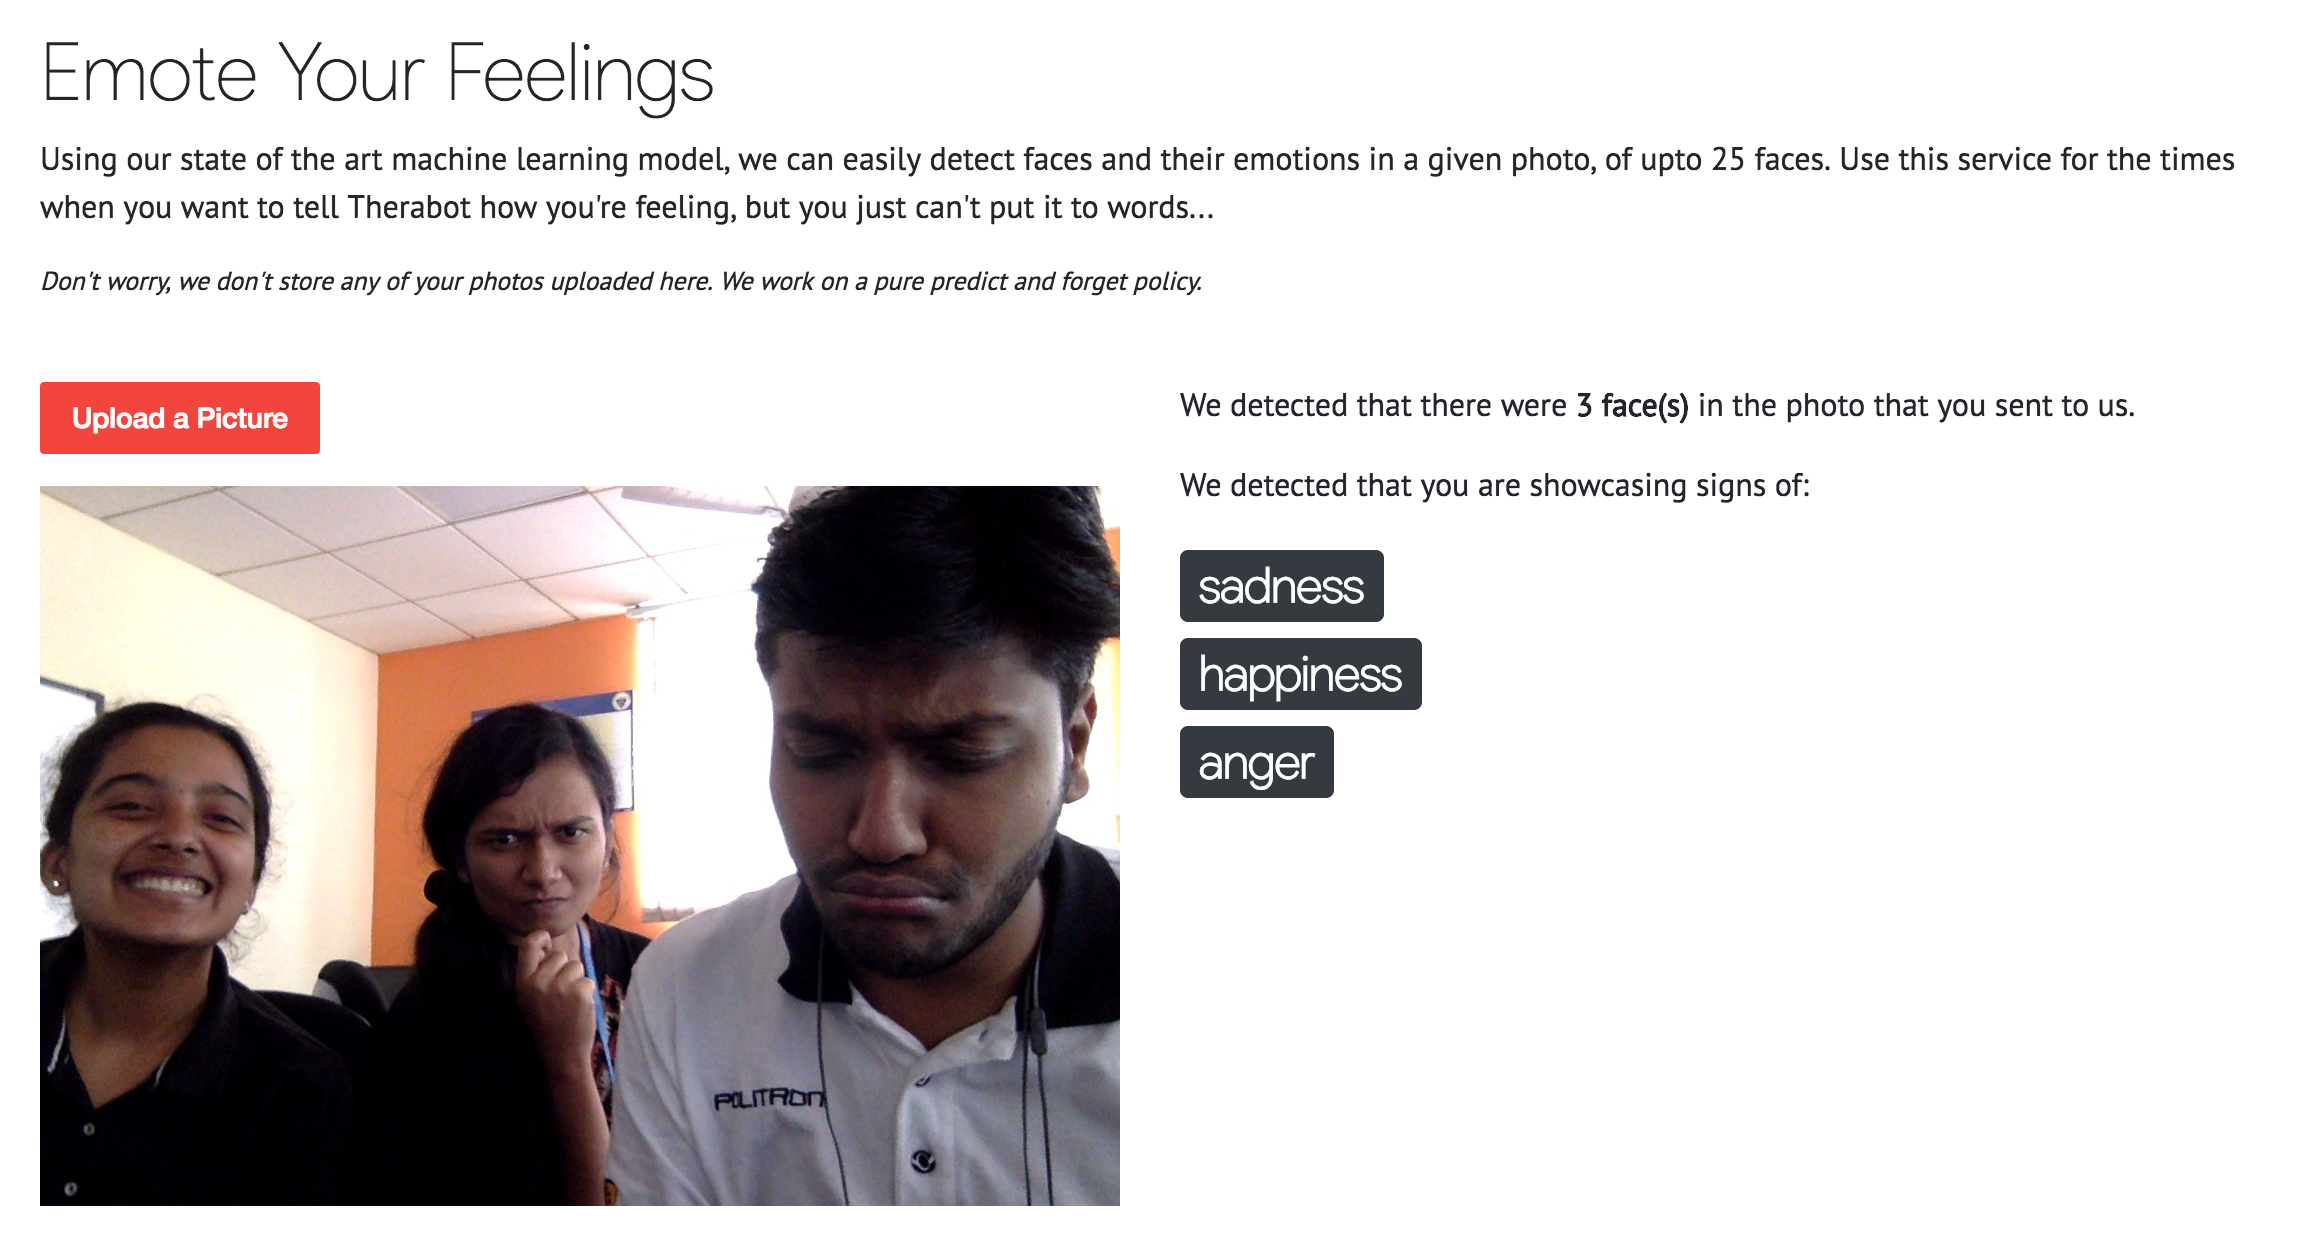
\includegraphics[width=6cm]{images/screenshots/website/website-emote-feelings.png}
    \caption{Module \#3 - Emote your Feelings}
\end{figure}

% Conclusion

\section{Conclusion}

From the product being built to the math behind the magic to how Therabot works, we can conclude successfully that we have stepped into a new field with respect to the marriage of mental wellness and artificial intelligence, where we can now use robotic speech and personalized speech generation to cater to the user and create a more lasting bond.

The stigma around depression and getting help from a medical professional is still very high, and we believe that with the ease of access to a personalized robotic therapist in your smartphones/laptops, it should make it much more easier to approach the concept of getting help. Through the course of marketing the idea, we noticed that a lot of people were open about the idea of talking to a non-human person about their feelings as opposed to a stranger.

We believe that with the right amount of question-answer datasets and user input, along with the prolonged reinforcement learning in place, we will be able to build a self-sustaining chatbot that can help at least the majority of people who are in need of a person to talk to.

% Acknowledgment

\section{Acknowledgment}

The satisfaction that accompanies the successful completion of our project would be incomplete without mentioning the people who made it possible, whose constant guidance and encouragement crowns all the efforts with success.

We would greatly mention the enthusiastic influence for provided by Dr. Krishnan R., Professor, Department of Computer of Science and Engineering of Dayananda Sagar College of Engineering for his ideas and co-operation during our venture and making this project a great success.

We are thankful to Dr. D. R. Ramesh Babu, Vice-Principal \& HoD of Department of Computer Science and Engineering of Dayananda Sagar College of Engineering for his co-operation during all phases of our project.

We are also thankful to Dr. C. P. S. Prakash, Principal of Dayananda Sagar College of Engineering, Bangalore for being kind enough to provide us an opportunity to work on a project in this institution.

It is a pleasure to thank the friendly co-operation showed by all the staff members of the Computer Science Department, Dayananda Sagar College of Engineering, and finally, not to forget our friends \& family who have supported us through our academic career.

\printbibliography

\end{document}